
\documentclass[%
 reprint,
%superscriptaddress,
%groupedaddress,
%unsortedaddress,
%runinaddress,
%frontmatterverbose, 
%preprint,
%showpacs,preprintnumbers,
%nofootinbib,   
%nobibnotes,
%bibnotes,
 amsmath,amssymb,
 aps,
%pra,
%prb,
%rmp,
%prstab,
%prstper,
%floatfix,
]{revtex4-1}

\usepackage{graphicx}% Include figure files
\usepackage{dcolumn}% Align table columns on decimal point
\usepackage{bm}% bold math
%\usepackage{hyperref}% add hypertext capabilities
%\usepackage[mathlines]{lineno}% Enable numbering of text and display math
%\linenumbers\relax % Commence numbering lines

%\usepackage[showframe,%Uncomment any one of the following lines to test 
%%scale=0.7, marginratio={1:1, 2:3}, ignoreall,% default settings
%%text={7in,10in},centering,
%%margin=1.5in,
%%total={6.5in,8.75in}, top=1.2in, left=0.9in, includefoot,
%%height=10in,a5paper,hmargin={3cm,0.8in},
%]{geometry}

\usepackage{siunitx}
\usepackage{color, soul}
\def\blue#1{\textcolor[rgb]{0,0,1}{#1}}
\def\red#1{\textcolor[rgb]{1,0,0}{#1}}
\usepackage{listings}
\usepackage{tikz}
\usetikzlibrary{trees}
\tikzstyle{every node}=[draw=black,thick,anchor=west]
\tikzstyle{selected}=[draw=red,fill=red!30]
\tikzstyle{optional}=[dashed,fill=gray!50]

\begin{document}

\preprint{APS/123-QED}

\title{VTAnDeM: A Python Toolkit for Visualizing Phase Stability, Defect Energetics, and Carrier Concentration in Materials}

\author{Michael Y. Toriyama$^{1,2}$}
\author{Jiaxing Qu$^{3}$}
\author{L\'idia Carvalho Gomes$^{4}$}
\author{Elif Ertekin$^{3,4,5}$}

\affiliation{$^{1}$Department of Materials Science and Engineering}
\affiliation{$^{2}$Department of Mathematics}
\affiliation{$^{3}$Department of Mechanical Engineering}
\affiliation{$^{4}$National Center for Supercomputing Applications}
\affiliation{$^{5}$Materials Research Laboratory, University of Illinois at Urbana-Champaign, Champaign, Illinois 61820, United States}

\date{\today}

\begin{abstract}
Phase stability, defect formation energies, and carrier concentrations are closely intertwined features of semiconductors. 
Due to their joint dependence on the multidimensional -- and often unintuitive --  chemical potential space, it is challenging to establish patterns and interrelationships between these quantities in a given semiconductor. 
To facilitate visualization and analysis of  these complementary material properties, we have developed the Visualization Toolkit for Analyzing Defects in Materials (VTAnDeM). 
This python-based toolkit allows users to interactively explore how defect formation energies and carrier concentrations vary across the chemical potential space from DFT data of complex multicomponent (ternary and quaternary) semiconductors.
We illustrate the computational workflow that employs VTAnDeM as a post-processing visualization tool, and describe the data organization and physical theory underlying the visualization scheme.
We anticipate that this developing software will serve as a back-end analysis toolkit that can readily interface with existing pre- and post-processing softwares for first-principles calculations to help researchers visualize the chemical potential -- defect -- carrier concentration phase space of complex semiconductors.
\end{abstract}

\maketitle

\section{Introduction}

%Phase stability and point defects underlie various mechanical, optical, and electronic properties of materials. In photovoltaics, intrinsic defects may contribute to electron-hole recombination mechanisms, which places an upper bound on the open-circuit voltage of bulk crystals [REF]. In structural materials, diffusion of atoms leading to mechanical deformation is contingent on point defects [REF]. Recent work on thermoelectric materials have determined that the electronic contribution to the figure of merit $zT$ is driven by defects, where dopability is closely tied to phase stability and defect tolerance of the material [REFs].

With various advancements in engineering and technology, the need for increasingly complex, multifunctional materials vitalizes the use of computational resources in materials engineering and design. Methods such as Density Functional Theory (DFT) and Molecular Dynamics (MD) have surged in recent years to provide crucial insights towards electronic structures and atomistic behaviors, helping to resolve various material properties that are either difficult or impossible to observe in an experimental setting. Material simulations have therefore witnessed numerous accomplishments and continue to expand in scope with waves of growing databases \cite{2013_Jain, 2013_Saal, 2016_Gorai, 2015_Kirklin} and developed post-processing softwares \cite{2013_Ong, 2017_Goyal, 2018_Broberg, 2018_Naik, 2018_Ward}.
%Computational approaches to materials research have therefore witnessed numerous accomplishments and continues to expand with waves of growing databases \cite{2013_Jain, 2013_Saal, 2016_Gorai, 2015_Kirklin} and developed post-processing softwares \cite{2013_Ong, 2017_Goyal, 2018_Broberg, 2018_Naik, 2018_Ward}.

%Although novel chemistries may be discovered through trial-and-error, methods such as Density Functional Theory (DFT) and Molecular Dynamics (MD) have surged in recent years to predict and tailor material properties \cite{2017_Gorai} [REFs]. Computational approaches to materials research has witnessed numerous accomplishments and continues to expand with growing databases \cite{2013_Jain, 2013_Saal, 2015_Gorai, 2015_Kirklin} and post-processing softwares \cite{2017_Goyal, 2018_Broberg, 2018_Ward}.

%With various advancements in fields where phase stability and defect engineering are crucial, increasingly complex, multicomponent material systems are being explored. Although novel chemistries may be discovered through various trial-and-error synthesis methods, the use of computational tools such as Density Functional Theory (DFT) have surged in recent years to predict and tailor material properties \cite{2017_Gorai} [REFs]. This data-oriented approach to materials research has witnessed numerous accomplishments [REFs] and continues to expand with growing databases [REF Materials Project, OQMD] and post-processing softwares [REFs]. Accordingly, post-processing tools for common DFT softwares are necessary for easily visualizing relevant material properties.

Point defects of materials in particular are extensively studied by computational means, which in turn have provided crucial insights towards various mechanical, optical, and electronic properties of materials. In photovoltaics, intrinsic defects often contribute to electron-hole recombination mechanisms, which places an upper bound on the open-circuit voltage of bulk crystals \cite{2014_Zakutayev, 2017_Kim, 2017_Liu, 2018_Liu, 2019_Kim}. Recent work on thermoelectric materials have determined that the electronic contribution to the figure of merit $zT$ is driven by the dopability of the material, which is closely tied to phase stability and defect tolerance of the material \cite{2008_Snyder, 2011_Pei, 2015_Yan}.

% In structural materials, diffusion of atoms leading to mechanical deformation is contingent on point defects [REF].

The stability of phases and defects in a material are both influenced by the chemical potential of each element in the material. Because of this, the two material properties are commonly plotted and reported in parallel \cite{2013_Chen, 2014_Chen, 2014_Tang, 2015_Swift, 2017_Adamski, 2017_Li, 2017_Zhu, 2019_Kim, 2019_Rowberg, 2019_Xu}. Softwares that post-process and visualize the phase stability and defect properties of a material from given data exist \cite{2014_Buckeridge, 2017_Pean, 2018_Stoliaroff}; yet, there are challenges associated with intuitively understanding how the phase stability of a material and defect formation energies directly depend on each other and on the chemical potential space. Accordingly, a post-processing software that visualizes both material properties \textit{simultaneously} in a coherent graphical user interface (GUI) would be useful, both from a computational and experimental standpoint.
%Although softwares that visualize phase stability and defect properties exist \cite{2014_Buckeridge, 2017_Pean, 2018_Stoliaroff}, none integrate a \textit{simultaneous} visualization capability of such closely interconnected material properties. Due to the challenges of intuitively understanding how the phase stability of a material and defect formation energies directly depend on the chemical potential space however, a visualization software that assimilates both material properties into a coherent graphical user interface (GUI) would be useful for further computational and experimental investigations.

In this report, we introduce the Visualization Toolkit for Analyzing Defects in Materials (VTAnDeM). This Python-based post-processing software is tailored specifically towards visualizing the stability and corresponding defect/electronic properties of ternary (3-component) and quaternary (4-component) materials. A summary of how VTAnDeM fits into the workflow of computational materials design is illustrated in Figure \ref{Figure:VTAnDeM_Overview}. We stress that softwares such as PyLaDa \cite{2017_Goyal} and PyCDT \cite{2018_Broberg} help to automate and post-process defect calculations of materials, and VTAnDeM is intended to act as a back-end visualization software once the DFT results are available.

%Some advantages of VTAnDeM over existing visualization softwares include:
%\begin{enumerate}
%\item material selectivity from a database compiled either by an individual user or the global community,
%\item simultaneous visualization of thermodynamic quantities coupled in real time by a user-explorable chemical potential space, and
%\item an extension of the phase stability visualization philosophy beyond ternary materials.
%\end{enumerate}

\begin{figure*}
\centering
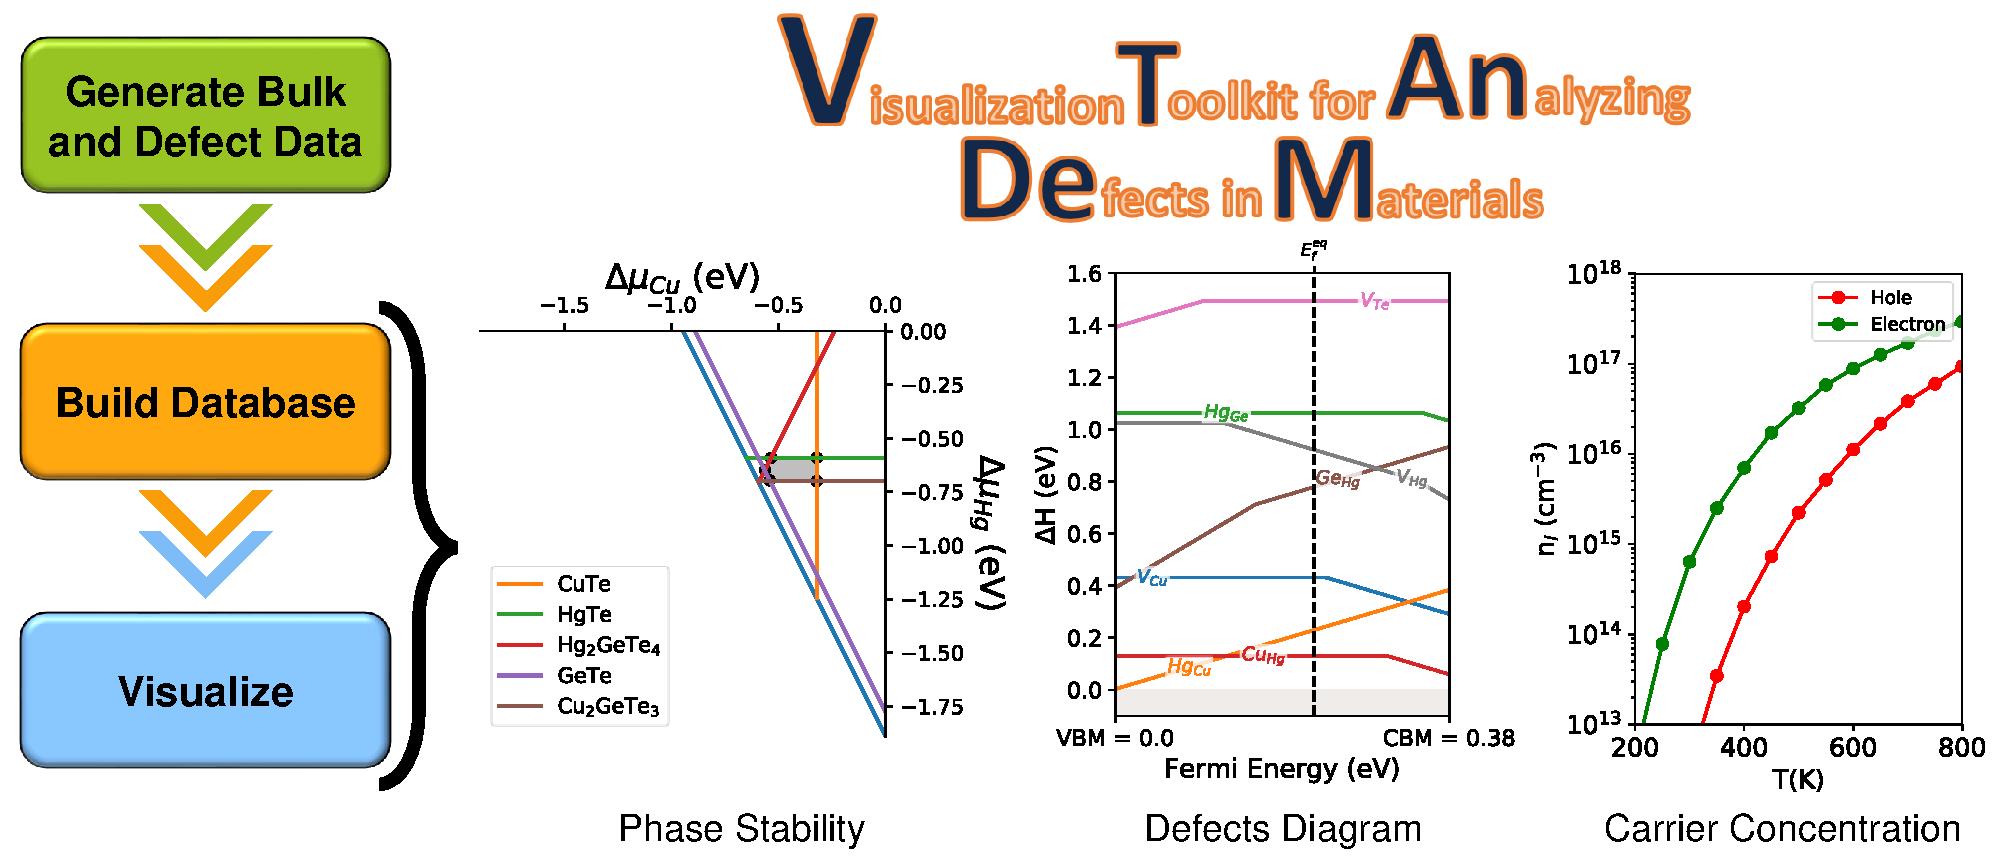
\includegraphics[scale=0.5]{VTAnDeM_Overview_v5.pdf}
\caption{Overview of VTAnDeM. 
VTanDeM is a post-processing tool for analysis of defect properties of semiconductors. 
Bulk materials properties and defect formation energies must be computed or otherwise available {\it a priori}. 
VTAnDeM imports these results and builds a database of relevant results based on user selections. 
%is intended to fit into the computational material analysis process and properties that are visualizable using VTAnDeM. 
It then provides interactive visualization of the interconnected thermodynamic/electronic properties of phase stability, defect formation energies, and carrier concentrations.}
\label{Figure:VTAnDeM_Overview}
\end{figure*}

The paper is organized as follows. In Section \ref{Section_WorkflowOverview}, we outline the basic workflow and provide a general overview of VTAnDeM's data organization. We then describe the mathematical treatment for visualizing the phase stability, defects diagram, and carrier concentration in Section \ref{Section_Theory}. We make concluding remarks and comment on future work in Section \ref{Section_Conclusion}.
%We outline in this paper the organization, usage, and the implemented theory of VTAnDeM. We outline the basic workflow and provide a general overview of VTAnDeM's data organization in Section \ref{Section_WorkflowOverview}. We then describe the mathematical treatment for visualizing the phase stability, defects diagram, and carrier concentration in Section \ref{Section_Theory}. We make concluding remarks and comment on future work in Section \ref{Section_Conclusion}.

We note that figures that show the phase stability, defects diagram, and carrier concentration are drawn using real DFT-generated data of Cu$_2$HgGeTe$_4$ (I$\overline{4}$2m). This quaternary compound has gained recent interest as a potential thermoelectric material due to its low lattice thermal conductivity and defect engineering possibilities \cite{2018_Ortiz, 2019_Ortiz, 2019_Gomes_InProgress, 2019_Qu_InProgress}. We therefore encourage that the figures be interpreted as an application of VTAnDeM towards analyzing thermodynamic/electronic properties of multicomponent materials.

%In this report, we introduce the Visualization Toolkit for Analyzing Defects in Materials (VTAnDeM). This Python-based post-processing software allows users to compile and visualize the phase stability diagram and defects diagram for ternary and quaternary materials in a streamlined manner. Although the outputs reproduce the plotting capabilities of existing softwares \cite{2017_Pean, 2018_Stoliaroff}, the main advantage of VTAnDeM is that the software can probe the entire accessible chemical potential space of ternary and quaternary materials in real-time. Furthermore, VTAnDeM can quickly produce the defects diagram and the corresponding temperature-dependent carrier concentration at any set of chemical potential values in phase space from DFT data.




\section{Workflow and Overview}
\label{Section_WorkflowOverview}

\subsection{Basic Workflow}
Each visual feature of VTAnDeM requires separate outputs from first-principles calculations, as shown in Figure \ref{Figure:Workflow}. To elaborate, the phase stability is determined by the total energies of the main ternary/quaternary material, as well as its competing compounds. The defects diagram is drawn from total energy calculations of possible point defects in the host ternary/quaternary material. The carrier concentration is drawn from the density of states (DOS) of the material.

Due to the fairly complicated set of inputs necessary to visualize the phase stability, defect formation energies, and carrier concentration of a material, a fixed workflow is maintained by VTAnDeM and explained below:

\begin{enumerate}

\item Initially, the user must create a VTAnDeM project in a directory of their choice.
\begin{verbatim}
mkdir ./project_directory
cd ./project_directory
vtandem --new
\end{verbatim}
This project folder is meant to compactify all data relevant to the specific material that the user is analyzing. As a result, the three files representing the user's portable database are initialized in this step, namely the \textit{Compounds\_Tracker.json}, \textit{Defects\_Tracker.json}, and \textit{DOS\_Tracker.json} files.

\item Next, the user must import all data relevant to the material, including bulk calculations of the elements, competing compounds, defect calculations, and DOS. This step is explained in further detail in Section \ref{Subsection:Importing_Data}.

\item Once the data has been imported, the user can visualize the quantities of interest using the command
\begin{verbatim}
vtandem --visualize
\end{verbatim}
in the project directory. Note that the user can only visualize quantities for which data has been supplied. For example, if defect calculations for a material has not been imported to the database, then neither the defects diagram nor the carrier concentration plots can be visualized.

\end{enumerate}

%As shown in Figure \ref{Figure:VTAnDeM_Overview}, the main features of VTAnDeM consist of visualizing the phase stability, defects diagram, and carrier concentration plot from user-provided DFT data. Each visual requires separate outputs from first-principles calculations. For the phase stability, the total energies of the main ternary/quaternary material, as well as its competing compounds, are necessary. The defects diagram is drawn from total energy calculations of possible defects in the host ternary/quaternary material. The carrier concentration is drawn from the density of states (DOS) of the material.

%As shown in Figure \ref{Figure:VTAnDeM_Overview}, VTAnDeM is built primarily for storing materials data and visualizing thermodynamic quantities. The DFT data is generated by the user, and an example workflow for the case of Cu$_2$HgGeTe$_4$ is shown in Figure \ref{Figure:Workflow}. Explicitly, the user's chronology is outlined as follows:

%The recommended user workflow is outlined in Figure \ref{Figure:Workflow} and explained below:
%\begin{enumerate}
%\item Initially, the user selects a ternary or quaternary material for which they want to understand the phase stability, defect formation properties, and the resulting temperature-dependent carrier concentration. The total energy for this compound (preferably by allowing ionic and volumetric relaxation) must be computed using first principles.
%\item Next, possible competing compounds of the ternary/quaternary material must be identified. This includes elemental compounds such as Cu and Te, as well as multicomponent compounds such as CuTe. A total energy calculation for each compound must be run, preferably with settings similar to the main material.
%\item For the ternary/quaternary material, point defects (vacancies, interstitials, antisites) must be identified and created. A total energy calculation for each defect complex must be calculated \textit{without volumetric relaxation}.
%\item A high-quality DOS is necessary to plot the carrier concentration accurately. A self-consistent calculation for the main material with a large number of bins for the DOS is recommended.
%\item Lastly, all generated data must be uploaded onto the VTAnDeM database.
%\end{enumerate}

\begin{figure*}
\centering
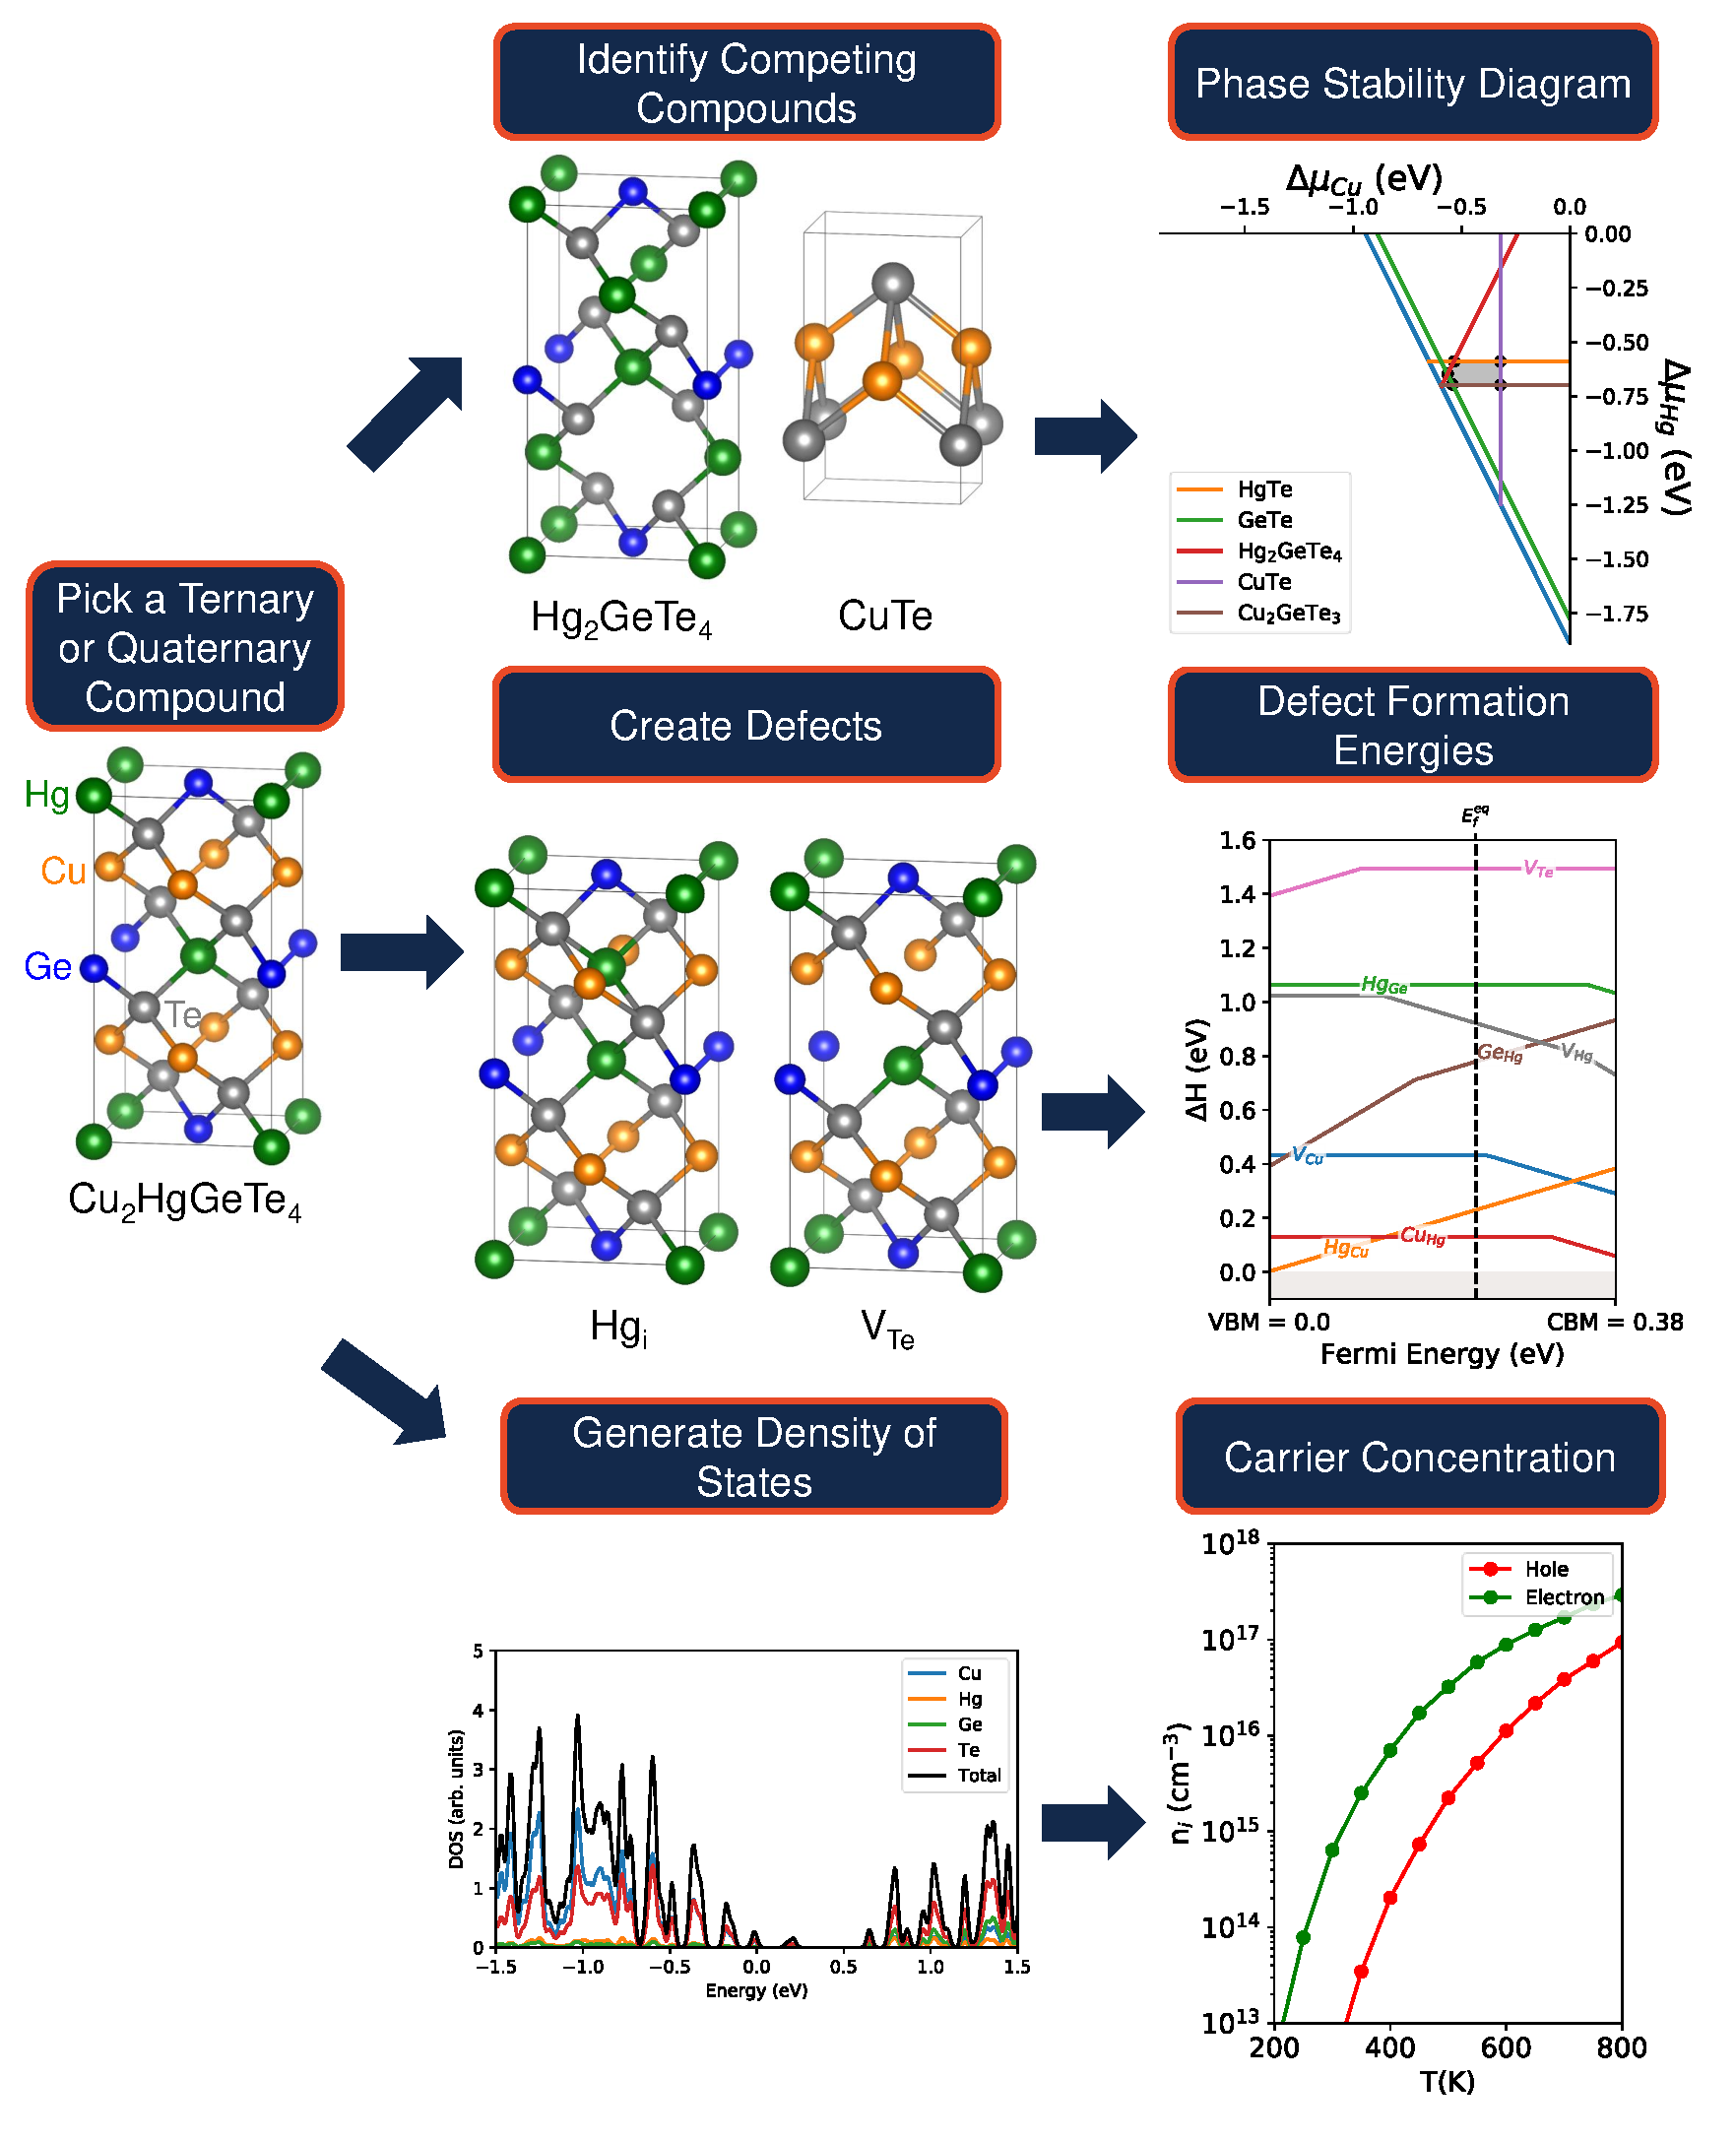
\includegraphics[width=0.835\textwidth]{Workflow_v6.pdf}
\caption{For a ternary/quaternary material of interest, the inputs that must be provided by the user to VTAnDeM are (i) the total energies of the material and all possible secondary competing compounds of interest, (ii) the formation energies of all defects of interest (including native defects and possibly extrinsic), and (iii) a high-quality density of states of the bulk compound. VTAnDeM uses these inputs to generate (i) phase stability diagrams in both chemical potential and composition space, and (ii) defect formation energy and (iii) carrier concentration diagrams generated on--the--fly for specific points in chemical potential space.}
\label{Figure:Workflow}
\end{figure*}
%Schematic of a VTAnDeM user's workflow. Once a ternary/quaternary material has been picked, find potential competing compounds consisting of elements included in the main material. These will constitute the thermodynamic stability of the material. Additionally, create point defects in the crystal structure of the main material. These calculations will feed into visualizing the defect properties of the material.


\subsection{Importing Data to the VTAnDeM Database} \label{Subsection:Importing_Data}

The user can upload data to the VTAnDeM database in one of three ways: using the GUI, the command line interface, or through the Python environment. Note that the current version of VTAnDeM can only read and post-process files generated by the Vienna Ab initio Simulation Package (VASP). However, as the software is further developed, we expect to have a version that supports other common DFT codes.


\subsubsection{Importing Data Using the GUI} \label{Subsubsection:Importing_Data_GUI}

A GUI is provided to guide the user when importing DFT data to the VTAnDeM database. The import dialog (Figure \ref{Figure:Upload_Interface}) can be called using the command 
\begin{verbatim}
vtandem --open
\end{verbatim}

The ``Import Compound Data'' option (Figure \ref{Figure:Upload_Interface}a) is used to import VASP outputs of bulk materials. Each bulk compound must be imported one at a time. The bulk elements must be imported before importing the data for bulk compound materials. The data directory for each material must contain files pertaining to the total energy of the material (either the OUTCAR or OSZICAR file), the number of atoms in the system (either the CONTCAR or POSCAR file), and the electronic structure of the material (the vasprun.xml file). The total energy of the system is extracted from the OUTCAR/OSZICAR file, normalized by the number of atoms as specified in the CONTCAR/POSCAR file. The band gap and valence band maximum are read from the vasprun.xml file using pymatgen \cite{2013_Ong}. These values pertaining to the electronic structure of the bulk material are used to draw the Fermi energy limits of the defect formation energy diagram. 

The ``Import Defects Data'' button (Figure \ref{Figure:Upload_Interface}b) is used to import data for a compound's various point defects. The defect type and its charge states that are recorded to the VTAnDeM database are determined by the names given to each folder. Accordingly, each defect must be represented by a folder with the name ``atom\_site'', and each charge state must be represented by subfolders with the name ``q\#'', where \# is the charge state. Additionally, the size of the supercell used in calculating the total energies of each defect, relative to the cell used in the bulk calculation of the compound, must be specified in the direction of each lattice vector.

Lastly, the ``Import DOS Data'' option (Figure \ref{Figure:Upload_Interface}c) is used to import the DOS of the bulk material. The DOS is extracted from the DOSCAR file. The DOS, along with the defect concentration, is used to determine the equilibrium Fermi energy by satisfying the charge neutrality condition. The electron and hole carrier concentrations are subsequently determined from the DOS and equilibrium Fermi energy.

%When importing bulk material data, VTAnDeM reads the total energy from the OUTCAR/OSZICAR file, the compound's stoichiometry from the POSCAR/CONTCAR file, and the band gap and valence band maximum from the vasprun.xml file. These three files must be included in a folder that is imported into VTAnDeM, as shown in Figure \ref{Figure:Upload_Interface}a. When importing defects data on the other hand, each defect must be represented by a folder with the name ``atom\_site''. The folder for a defect should contain separate folders representing each charge state with name ``q\#'', where \# is the charge state. As shown in Figure \ref{Figure:Upload_Interface}b, each ``q\#'' folder should contain the OUTCAR/OSZICAR file containing the total energy of the calculation. The DOS of the material can be directly imported from the DOSCAR file as shown in Figure \ref{Figure:Upload_Interface}c.

\begin{figure}
\centering
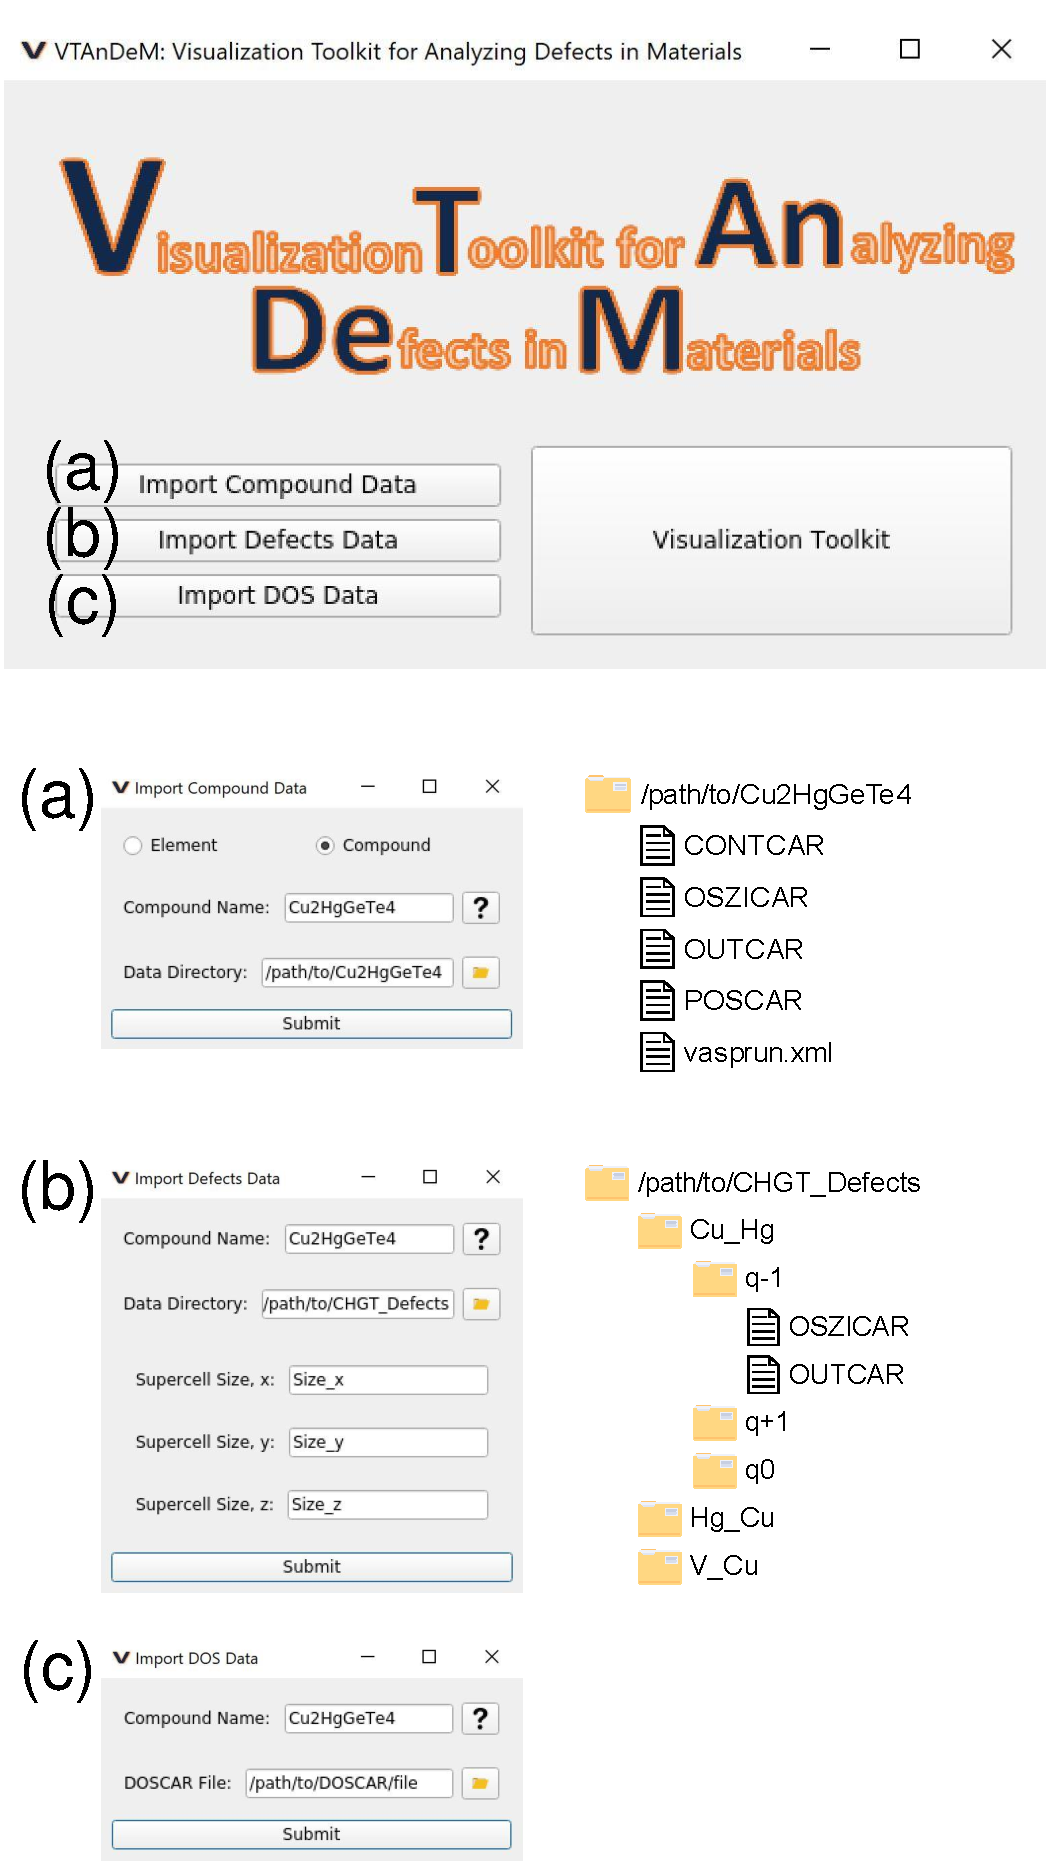
\includegraphics[scale=0.45]{Upload_Interface_v4.pdf}
\caption{Initial dialog when VTAnDeM is launched. The options on the left are used to import specific data types into the VTAnDeM database: (a) bulk material data, both for elemental and compound materials, (b) point defects for a specific material, and (c) the DOS of the material.}
\label{Figure:Upload_Interface}
\end{figure}


\subsubsection{Importing Data Using the Command Line} \label{Subsubsection:Importing_Data_CL}

The second method for importing DFT data into the VTAnDeM database is by using the command line directly. The bulk elements must be imported first using the syntax
\begin{verbatim}
vtandem --import_element NAME PATH
\end{verbatim}
where \verb+NAME+ is the name of the element (e.g. \verb+Cu+) and \verb+PATH+ is the path to the directory containing the OUTCAR/OSZICAR, CONTCAR/POSCAR, and vasprun.xml files. The \verb+PATH+ argument can be either the absolute or relative path. Once each element has been imported, the main ternary/quaternary compound, along with its competing compounds, can be imported with the slightly different command
\begin{verbatim}
vtandem --import_compound NAME PATH
\end{verbatim}
where \verb+NAME+ refers to the compound name (e.g. \verb+Cu2HgGeTe4+) and \verb+PATH+ is the path to the data directory. It is crucial that the elemental bulk systems be imported \textit{before} any compound materials are imported to the database.

The point defect calculations for a ternary/quaternary material may be imported using the command
\begin{verbatim}
vtandem --import_defects NAME PATH X Y Z
\end{verbatim}
where \verb+NAME+ is the compound name as before, the variable \verb+PATH+ is the path to the data directory as organized to the right of Figure \ref{Figure:Upload_Interface}b, and the arguments \verb+X+, \verb+Y+, and \verb+Z+ refer to the size of the supercell in the directions of the three lattice vectors, relative to the unit cell size of the bulk material. For example, if the supercell has the size 2x3x1 relative to the undefected system, (\verb+X+, \verb+Y+, \verb+Z+) = (2, 3, 1).

Lastly, the DOS may be imported into the VTAnDeM database with the command 
\begin{verbatim}
vtandem --import_dos NAME DOSCAR_PATH
\end{verbatim}
where \verb+DOSCAR_PATH+ is the path of the DOSCAR file, including the file name as in Figure \ref{Figure:Upload_Interface}c.


\subsubsection{Importing Data Using a Python Script} \label{Subsubsection:Importing_Data_Python}

The third method for importing data into the VTAnDeM database is through the Python environment. The chronology is similar to the other two importing methods: import the bulk elements, the main compound and competing compounds, the point defects for the main compound, and lastly the DOS for the main compound. This can be done with a single script.

The command for importing bulk elements and compounds is
\begin{verbatim}
from vtandem.dft import import_dft
x = import_dft.Compounds_Import()
x.Add_Element(`NAME', `PATH')
x.Add_Compound(`NAME', `PATH')
x.Update_Compounds_Database()
\end{verbatim}
where \verb+import_dft.Compounds_Import()+ initializes a class with methods \verb+Add_Element+, \verb+Add_Compound+, and \verb+Update_Compounds_Database+. The arguments \verb+NAME+ and \verb+PATH+ are defined as in Section \ref{Subsubsection:Importing_Data_CL}.

Subsequently, point defect calculations may be imported into the VTAnDeM database with the syntax
\begin{verbatim}
y = import_dft.Defects_Import()
y.Add_Defects(`NAME', `PATH', X, Y, Z) 
y.Update_Defects_Database()
\end{verbatim}

Lastly, the DOS may be imported with the command
\begin{verbatim}
z = import_dft.DOS_Import()
z.Add_DOS(`NAME', `DOSCAR_PATH')
z.Update_DOS_Database()
\end{verbatim}





%The second method for importing DFT data into the VTAnDeM database is to manually enter the necessary quantities. This method allows flexibility for the user in several ways. Firstly, the user can specify quantities such as the enthalpy of formation or band gap when only an approximate or experimental value is given. Moreover, manually entering the defects data allows users to implement a correction scheme of their choice. Given that only VASP output files are supported by VTAnDeM, data from other DFT codes may also be entered manually into the database.



\subsection{VTAnDeM Data Structure} \label{Subsection:Data_Structure}

VTAnDeM's data structure is organized into three separate libraries: one for visualizing the phase stability (\textit{Compounds\_Tracker.json}), another for visualizing the defects diagram (\textit{Defects\_Tracker.json}), and a third for visualizing the carrier concentration (\textit{DOS\_Tracker.json}).

\begin{figure*}
    \centering
    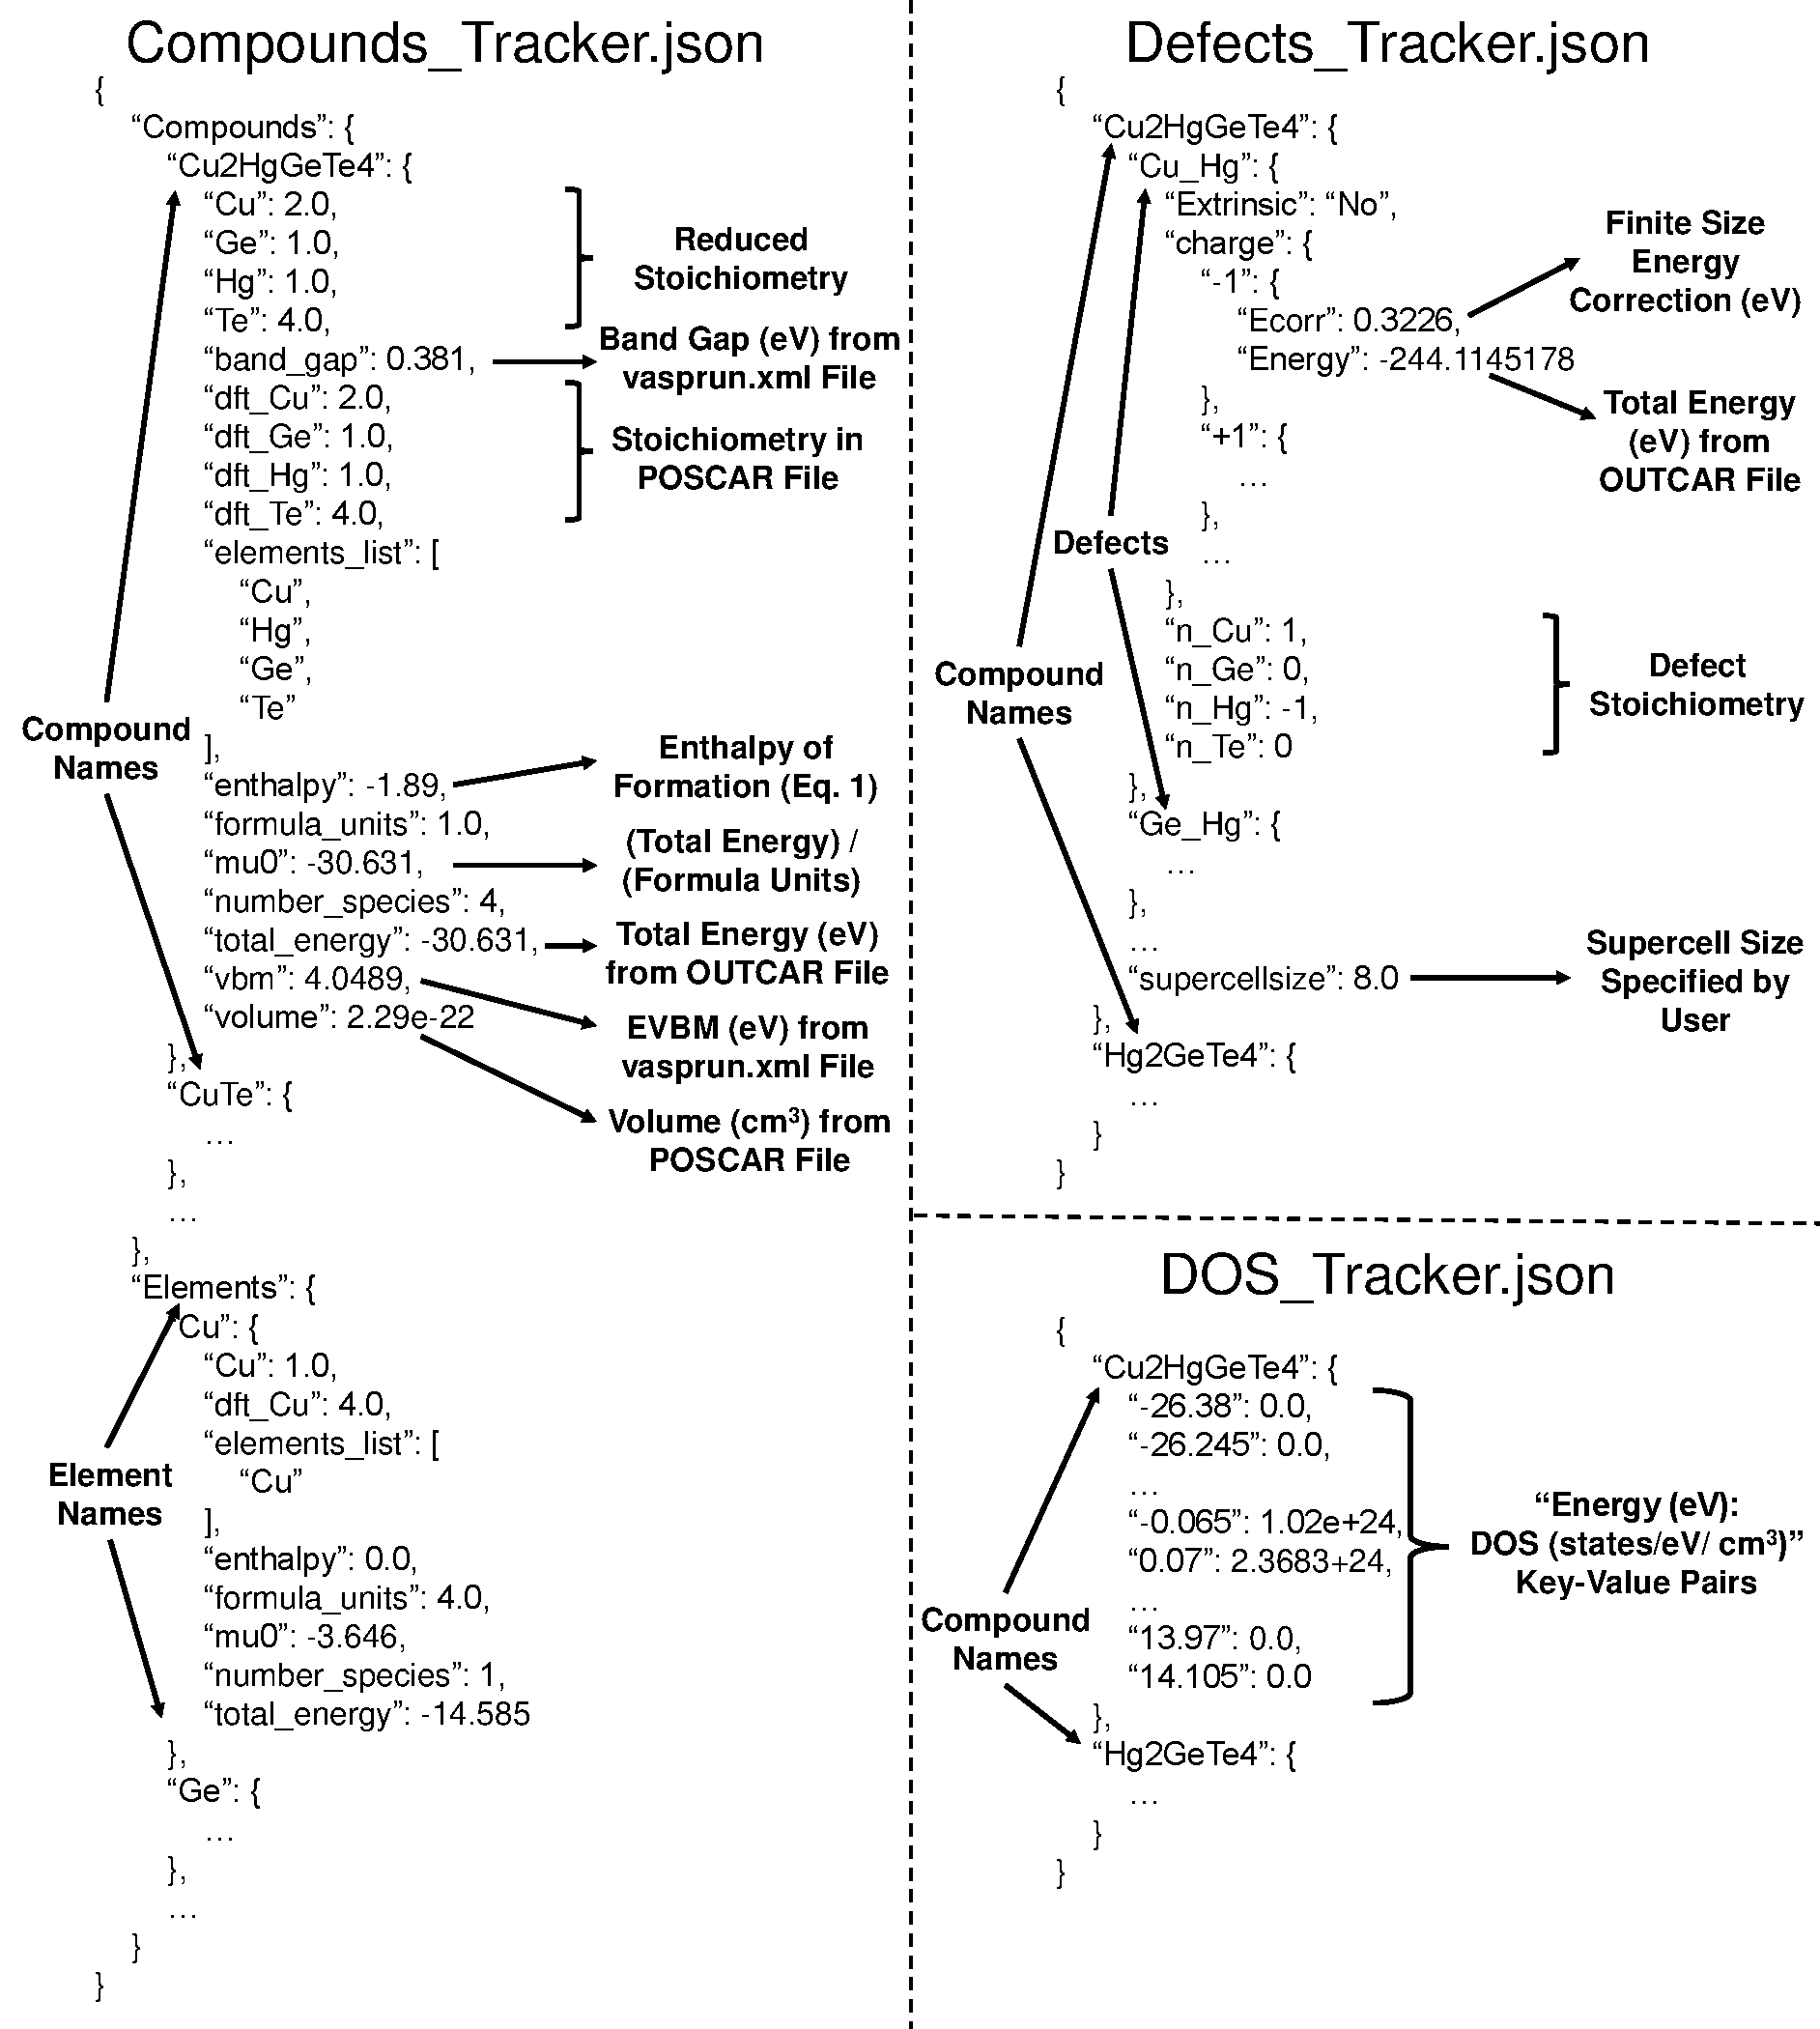
\includegraphics[width=0.8\textwidth]{DataStructure.pdf}
    \caption{VTAnDeM's internal data structure for (left) bulk material and (right) defect related information.}
    \label{Figure:VTAnDeM_DataStructure}
\end{figure*}

The \textit{Compounds\_Tracker.json} file stores chemical and thermodynamic information about the main ternary/quaternary material, its constituent elements, and competing compounds of the material. The data is organized as shown in the left column of Figure \ref{Figure:VTAnDeM_DataStructure}. We note that a crucial piece of information needed to draw the phase stability diagram is the enthalpy of formation of each compound, which is internally computed by VTAnDeM using the chemical potentials of each element. Therefore, it is important for the user to import data for the elemental species before importing compounds data. As an example, before importing the information for Cu$_2$HgGeTe$_4$, the user must import the DFT data for Cu, Hg, Ge, and Te.

The \textit{Defects\_Tracker.json} file contains energetic properties of possible defects in ternary/quaternary materials stored in the \textit{Compounds\_Tracker.json} file. The total energy and finite-size corrections are recorded for each charge state of each defect as shown in the top-right column of Figure \ref{Figure:VTAnDeM_DataStructure}. Currently, finite-size corrections are not computed by VTAnDeM and are recorded as ``0.0'' when defects data are imported. This feature however is under development and should be expected in future versions of the software.

Lastly, the \textit{DOS\_Tracker.json} file is simply organized into key-value pairs of the energy and corresponding DOS, as shown in the bottom right column of Figure \ref{Figure:VTAnDeM_DataStructure}. The recorded DOS values are normalized to the unit cell volume and are in units of $cm^{-3}$.

We note that since the VTAnDeM database is composed of alterable files, a user may manually enter the necessary quantities. This method allows flexibility for users in several ways. Firstly, the user can specify quantities when an approximate or experimental value is given. Moreover, the user can manually enter a correction value for the defect formation energy using a scheme of their choice. Data from other DFT codes may also be entered manually into the database.


%\subsubsection{Compounds\_Tracker.json} \label{Subsubsection:Compounds_Tracker}
%The \textit{Compounds\_Tracker.json} file stores chemical and thermodynamic information about the main ternary/quaternary material, its constituent elements, and competing compounds of the material. The data is organized as in Figure \ref{Figure:} \textcolor{red}{Add example table for Cu2HgGeTe4 to illustrate tabular structure?}, as each relevant property is recorded for every element and compound. The data is stored in the \textit{Compounds\_Tracker.json} file. 

%We highlight that this single file may hold information for as many DFT calculations as the user wishes, as VTAnDeM is built to generate the phase stability diagram of a given material using only the information of compounds that are considered ``competing''. In particular, the unrestricted data storage infrastructure allows VTAnDeM to be used as a scalable visualization software that can interface with large-scale material databases.

%\subsubsection{Defects\_Tracker.json} \label{Subsubsection:Defects_Tracker}

%The second library contains energetic properties of possible defects in the ternary/quaternary materials listed in \textit{Compounds\_Tracker.csv}. The total energy and finite-size corrections are recorded for each charge state of each defect. Since not all defects attain the same charge state, a tabular data structure demanding a DFT calculation for a fixed set of charge states would not be optimal; instead, the data is organized in a tree structure as a JSON file, called \textit{Defects\_Tracker.json}. \textcolor{red}{Add example tree structure of illustrate data structure?}



\subsection{Graphical User Interface}

The user is initially introduced to a material selection dialog listing the available ternary/quaternary materials in the \textit{Compounds\_Tracker.json} library (Figure \ref{Figure:VTAnDeM_VisualizationCapabilities}a). Defects and DOS data for these compounds need \textit{not} be provided to launch VTAnDeM; instead, VTAnDeM will show the plots that it can generate based on the available data. Once a material has been selected, the user can navigate between three visualization tabs.

The first tab (Figure \ref{Figure:VTAnDeM_VisualizationCapabilities}b) contains, at most, three side-by-side windows showing the projected phase stability region, defects diagram, and the temperature-dependent carrier concentration of the selected material, depending on which data is available. The chemical potential axes of the phase diagram can be changed using the dropdown menus located below the diagram. The three diagrams are interconnected through the user-tunable chemical potentials of the elemental species in the material. The user can explore this chemical potential space by clicking on the phase stability window, editing the text boxes, or using the slider (for quaternary compounds), and the defects diagram and carrier concentration plot will change accordingly in real time. In the defects diagram, the user can specify the temperature at which the defects are synthesized (denoted $T_{syn}$), which will change the defect concentration and hence alter the electron and hole carrier concentrations satisfying the charge neutrality condition. Provided that data for extrinsic dopants exist in \textit{Defects\_Tracker.json}, the user may also view how a dopant atom affects the equilibrium Fermi energy and carrier concentration of the material. In the carrier concentration plot, the user may specify the ambient temperature to observe how the equilibrium Fermi energy shifts in the band gap of the material.

The second tab (Figure \ref{Figure:VTAnDeM_VisualizationCapabilities}c) exhibits an interactive three-dimensional representation of the stability region of the material in chemical potential space. The user will see which competing compounds form facets in the stability region of the material. A slice of the convex polytope, dictated by the chemical potential of the fourth (dependent) species tunable by the slider bar, is projected to the three pairs of chemical potential axes shown to the right. Lastly, the third tab (Figure \ref{Figure:VTAnDeM_VisualizationCapabilities}d) exhibits the phase diagram in composition space, as opposed to the diagram being drawn in chemical potential space. VTAnDeM utilizes the pymatgen.analysis.phase\_diagram module to draw the compositional phase diagram \cite{2013_Ong}.

%The phase stability region is defined by a solid for quaternary materials (three independent and one dependent variables), whereas the stabilty region is defined by a plane for ternary materials (two independent and one dependent variables). As such, the projections can vary with the chemical potential of the dependent element for quaternary materials, which fixes a plane in the solid phase stability region. On the other hand, the projections do not vary for ternary materials.

%The third tab (Figure \ref{Figure:VTAnDeM_VisualizationCapabilities}d) exhibits an interactive phase diagram in composition space. The calculation is performed by Pymatgen \cite{2013_Ong}.

Note that snapshots of the VTAnDeM GUI shown in Figure \ref{Figure:VTAnDeM_VisualizationCapabilities} are an example visualization of a \textit{quaternary} material. The diagrams will look different for ternary materials however. For example, the slider in the first and second tabs (Figure \ref{Figure:VTAnDeM_VisualizationCapabilities}b,c) will not exist for ternary compounds. In the second tab (Figure \ref{Figure:VTAnDeM_VisualizationCapabilities}c), the three-dimensional representation of the phase stability region for a ternary material will be a plane for ternary materials (two independent and one dependent variables) instead of a solid for quaternary materials (three independent and one dependent variables). Accordingly, the competing compounds will form edges on planar phase stability region for ternary materials instead of facets. In the third tab (Figure \ref{Figure:VTAnDeM_VisualizationCapabilities}d), the compositional phase diagram will only have three vertices, one for each of the three elements in a ternary compound, and will hence be a two-dimensional triangle instead of a tetrahedron.

\begin{figure}
    \centering
    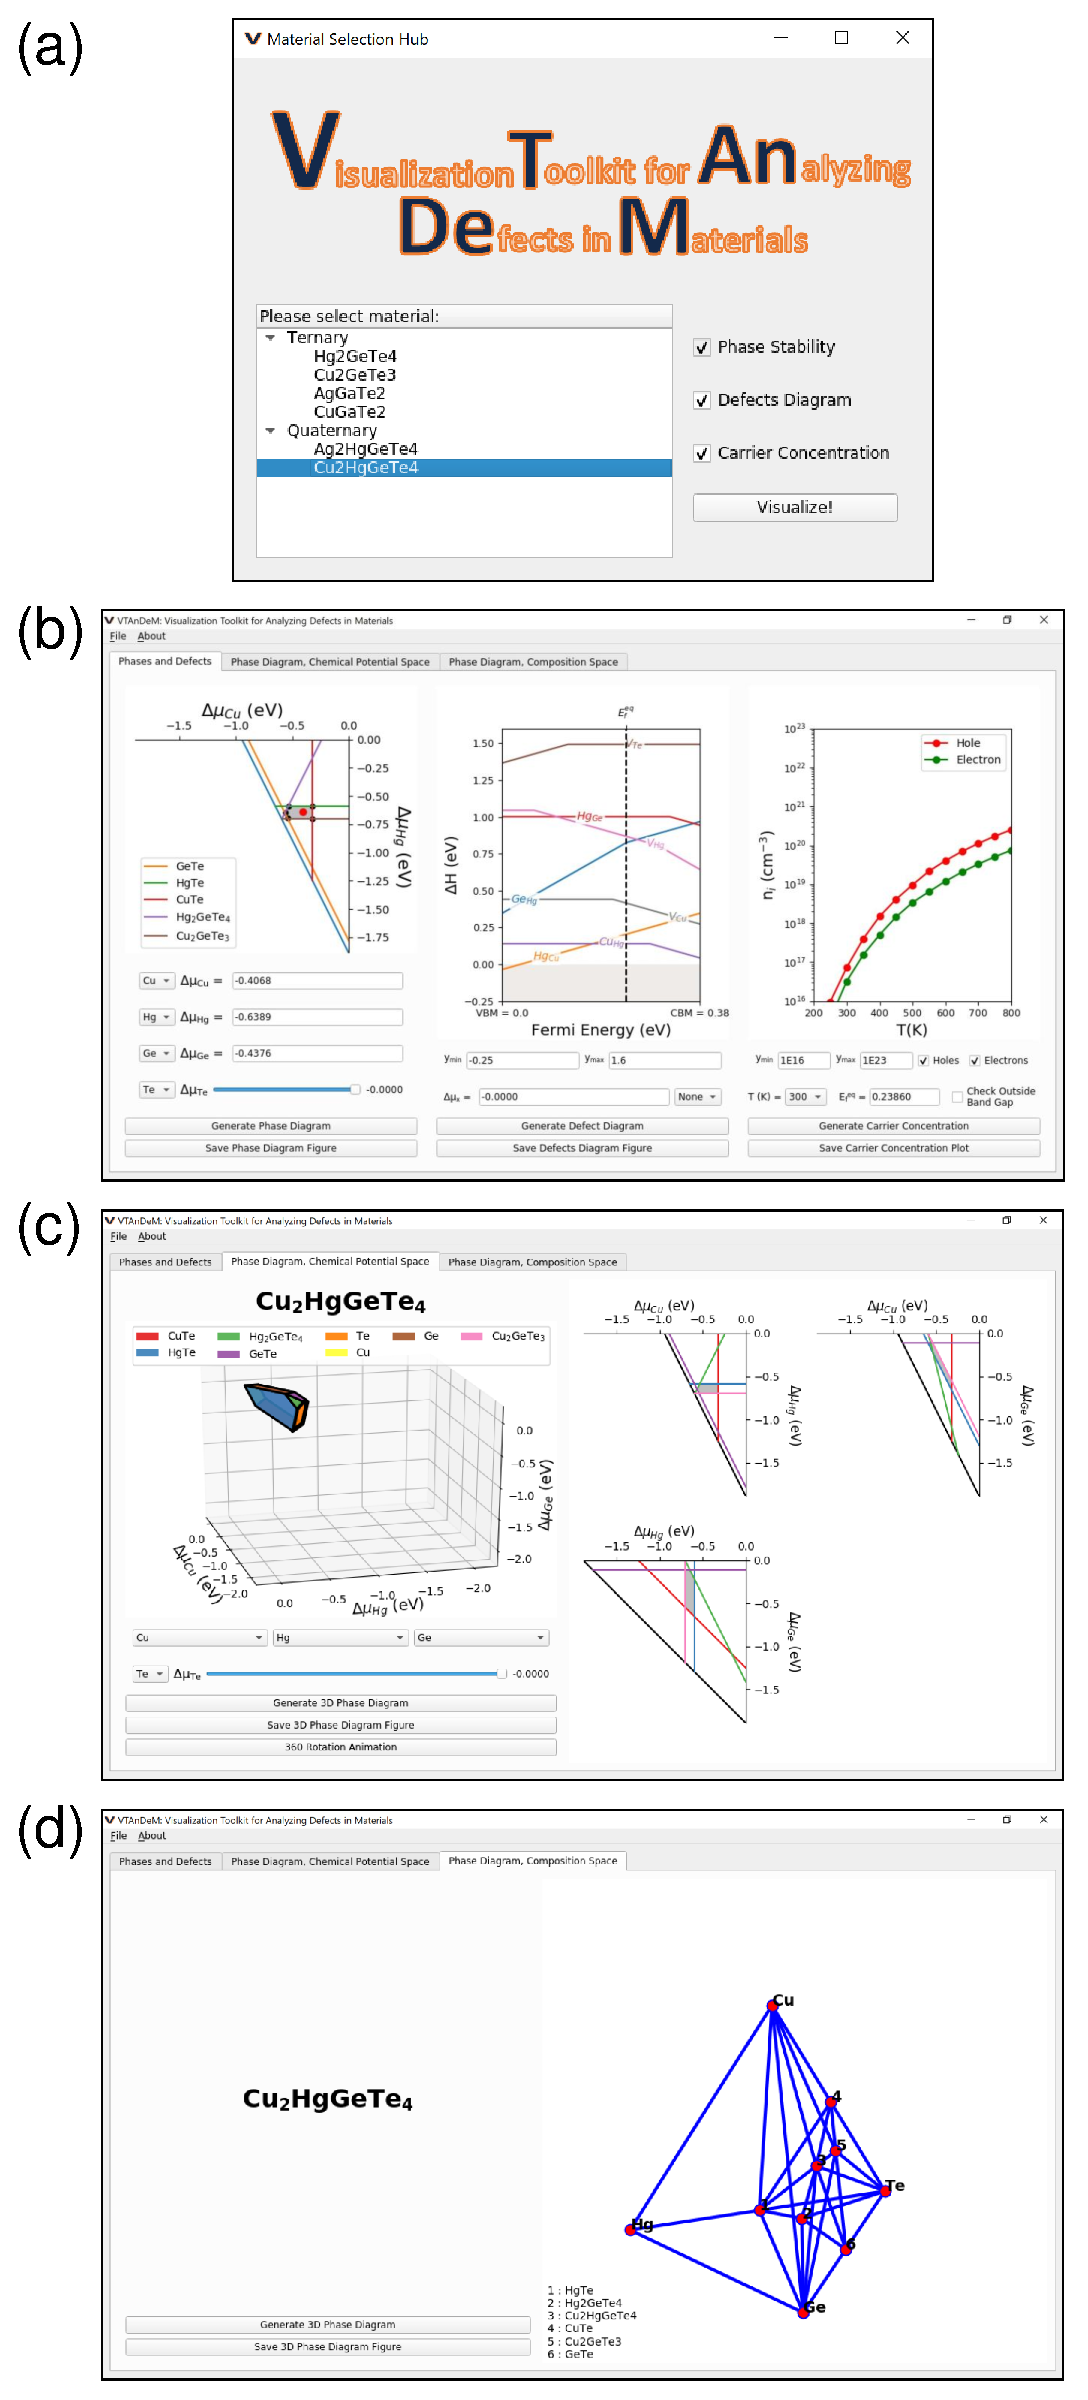
\includegraphics[scale=0.475]{VTAnDeM_VisualizationCapabilities_v4.pdf}
    \caption{The four interactive windows of VTAnDeM's visualization capabilities. (a) Initial launch of the visualization toolkit will prompt selection of a ternary/quaternary material. (b) Side-by-side plots of the phase stability diagram projected onto two chemical potential axes, the defect formation energy diagram, and carrier concentration. (c) The phase stability diagram shown with respect to three chemical potential axes. (d) Visualization of the phase diagram in composition space, incorporated via pymatgen \cite{2013_Ong}.}
    \label{Figure:VTAnDeM_VisualizationCapabilities}
\end{figure}



\section{Theory} \label{Section_Theory}

\subsection{Phase Stability in Chemical Potential Space}
The stability of a material is governed by thermodynamic principles underlying its chemistry. For an $n$-ary material $M = A^1_{a_1} A^2_{a_2}...A^n_{a_n}$, where $A^i$ is the $i^{th}$ element in the material and $a_i$ defines the stoichiometry, the enthalpy of the material $H_M$ is given by
\begin{align} \label{Equation:ChemPotEq}
H_M = \sum_i a_i \mu_{A^i}.
\end{align}
The chemical potential $\mu_{A^i}$ of element $A^i$ is the sum of an intrinsic and extrinsic contribution to the potential defined by
\begin{align} \label{Equation:ChemPotDef}
\mu_{A^i} = \mu^{\circ}_{A^i} + \Delta \mu_{A^i},
\end{align}
where $\mu^{\circ}_{A^i}$ is the intrinsic chemical potential of a single $A^i$ atom and $\Delta \mu_{A^i} \leq 0$ is the external contribution from the chemical environment. We refer to a more negative $\Delta \mu_{A^i}$ as an $A^i$-poor environment and, in contrast, a less negative $\Delta \mu_{A^i}$ as an $A^i$-rich environment.

The stability of a material is quantified by the enthalpy of formation ($\Delta H^M_{\text{f}}$) of the material, which is defined by
\begin{equation}
\begin{aligned}
\Delta H^M_{\text{f}} & = H_M - \sum_i a_i \mu^{\circ}_{A^i} \\
& = \sum_i a_i \Delta \mu_{A^i}.
\end{aligned}
\label{Equation:EnthalpyFormation}
\end{equation}
This notion can be rationalized in the following way: since we assume that the material $M$ (product) is formed from its constituent elements in their bulk phases (reactants), the tendency for $M$ to form, $\Delta H^M_{\text{f}}$, is the difference between the enthalpies of the product and reactants. Fortunately, $H_M$ and $\mu^{\circ}_{A^i}$ are the ground state energies per formula unit at zero kelvin and are therefore calculable using DFT.

Since multicomponent materials are composed of two or more distinct chemical species ($n \geq 2$), it is possible that undesirable ``competing compounds'' with chemical formula $C_j = A^1_{b^j_1} A^2_{b^j_2} ... A^m_{b^j_m}$ may form during synthesis of $M$, where $A^i$ and $b^j_i$ are the $i^{th}$ chemical species and stoichiometry, respectively, of the $j^{th}$ competing compound. $C_j$ will form more favorably than $M$ when its enthalpy of formation, $\Delta H^{C_j}_{\text{f}}$, is more negative than $\Delta H^{M}_{\text{f}}$. Equivalently, $M$ is stable when the formation enthalpy of \textit{each} competing compound satisfies
\begin{equation}
\begin{aligned}
\Delta H^{C_j}_{\text{f}} & = H_{C_j} - \sum_{i} b_i \mu^{\circ}_{A^i} \\
& \geq \sum_i b_i \Delta \mu_{A^i}.
\end{aligned}
\label{Equation:EnthalpyFormationCompeting}
\end{equation}
The stability region of an $n$-ary material $M$ is therefore constrained by a set of linear inequalities with at most $(n-1)$ degrees of freedom.

%This will occur in chemical environments where an excess/deficient amount of elements are found. In such situations, ``competing compounds'' with chemical formula $C^j = A^1_{b^j_1} A^2_{b^j_2} ... A^m_{b^j_m}$ will form, where $A^i$ and $b^j_i$ are the $i^{th}$ chemical species and stoichiometry, respectively, of the $j^{th}$ competing compound. It is worth noting that $C_j$ is considered a competing compound of $M$ only if each species $A^i$ exists in $M$, since we are not assuming any impurities in the phase diagram.
%The material of interest $M$ may not form in certain chemical environments however, due to driving forces introduced by excess/deficient amounts of certain chemical species. In such situations, ``competing compounds'' with formula $C^j = A^1_{b^j_1} A^2_{b^j_2} ... A^m_{b^j_m}$ will form, where $A^i$ and $b^j_i$ are the $i^{th}$ chemical species and stoichiometry, respectively, of the $j^{th}$ competing compound. It is worth noting that $C_j$ is considered a competing compound of $M$ only if each species $A^i$ exists in $M$, since we are not assuming any impurities in the phase diagram.
%However, complications arise when increasingly complex, multicomponent chemistries with $n \geq 3$ are considered. This is due to the possibility of forming ``competing compounds'' with formula $C^j = A^1_{b^j_1} A^2_{b^j_2} ... A^m_{b^j_m}$, where $A^i$ and $b^j_i$ are the $i^{th}$ chemical species and stoichiometry, respectively, of the $j^{th}$ competing compound. Note that $C_j$ may only be considered a competing compound of $M$ if each species $A^i$ coincide with those in $M$, since we are not assuming any impurities in the phase diagram.

An example of how competing compounds define the stability region of the quaternary material Cu$_2$HgGeTe$_4$ is shown in Figure \ref{Figure:PhaseStability_Schematic}. By considering only the formation of bulk elemental phases, the stability region is defined by Equation (\ref{Equation:EnthalpyFormation}) bounded by $\Delta \mu_{\text{Cu}}, \Delta \mu_{\text{Hg}}, \Delta \mu_{\text{Ge}}, \Delta \mu_{\text{Te}} \leq 0$ as in Equation (\ref{Equation:EnthalpyFormationCompeting}). The resulting phase stability region is shown in Figure \ref{Figure:PhaseStability_Schematic}a. As multicomponent competing compounds such as CuTe and Hg$_2$GeTe$_4$ are considered, new facets are introduced until the final phase stability region of Cu$_2$HgGeTe$_4$ emerges as in Figure \ref{Figure:PhaseStability_Schematic}b. The color of each facet corresponds to the element/compound that introduces the stability region bound.

\begin{figure}[ht]
    \centering
    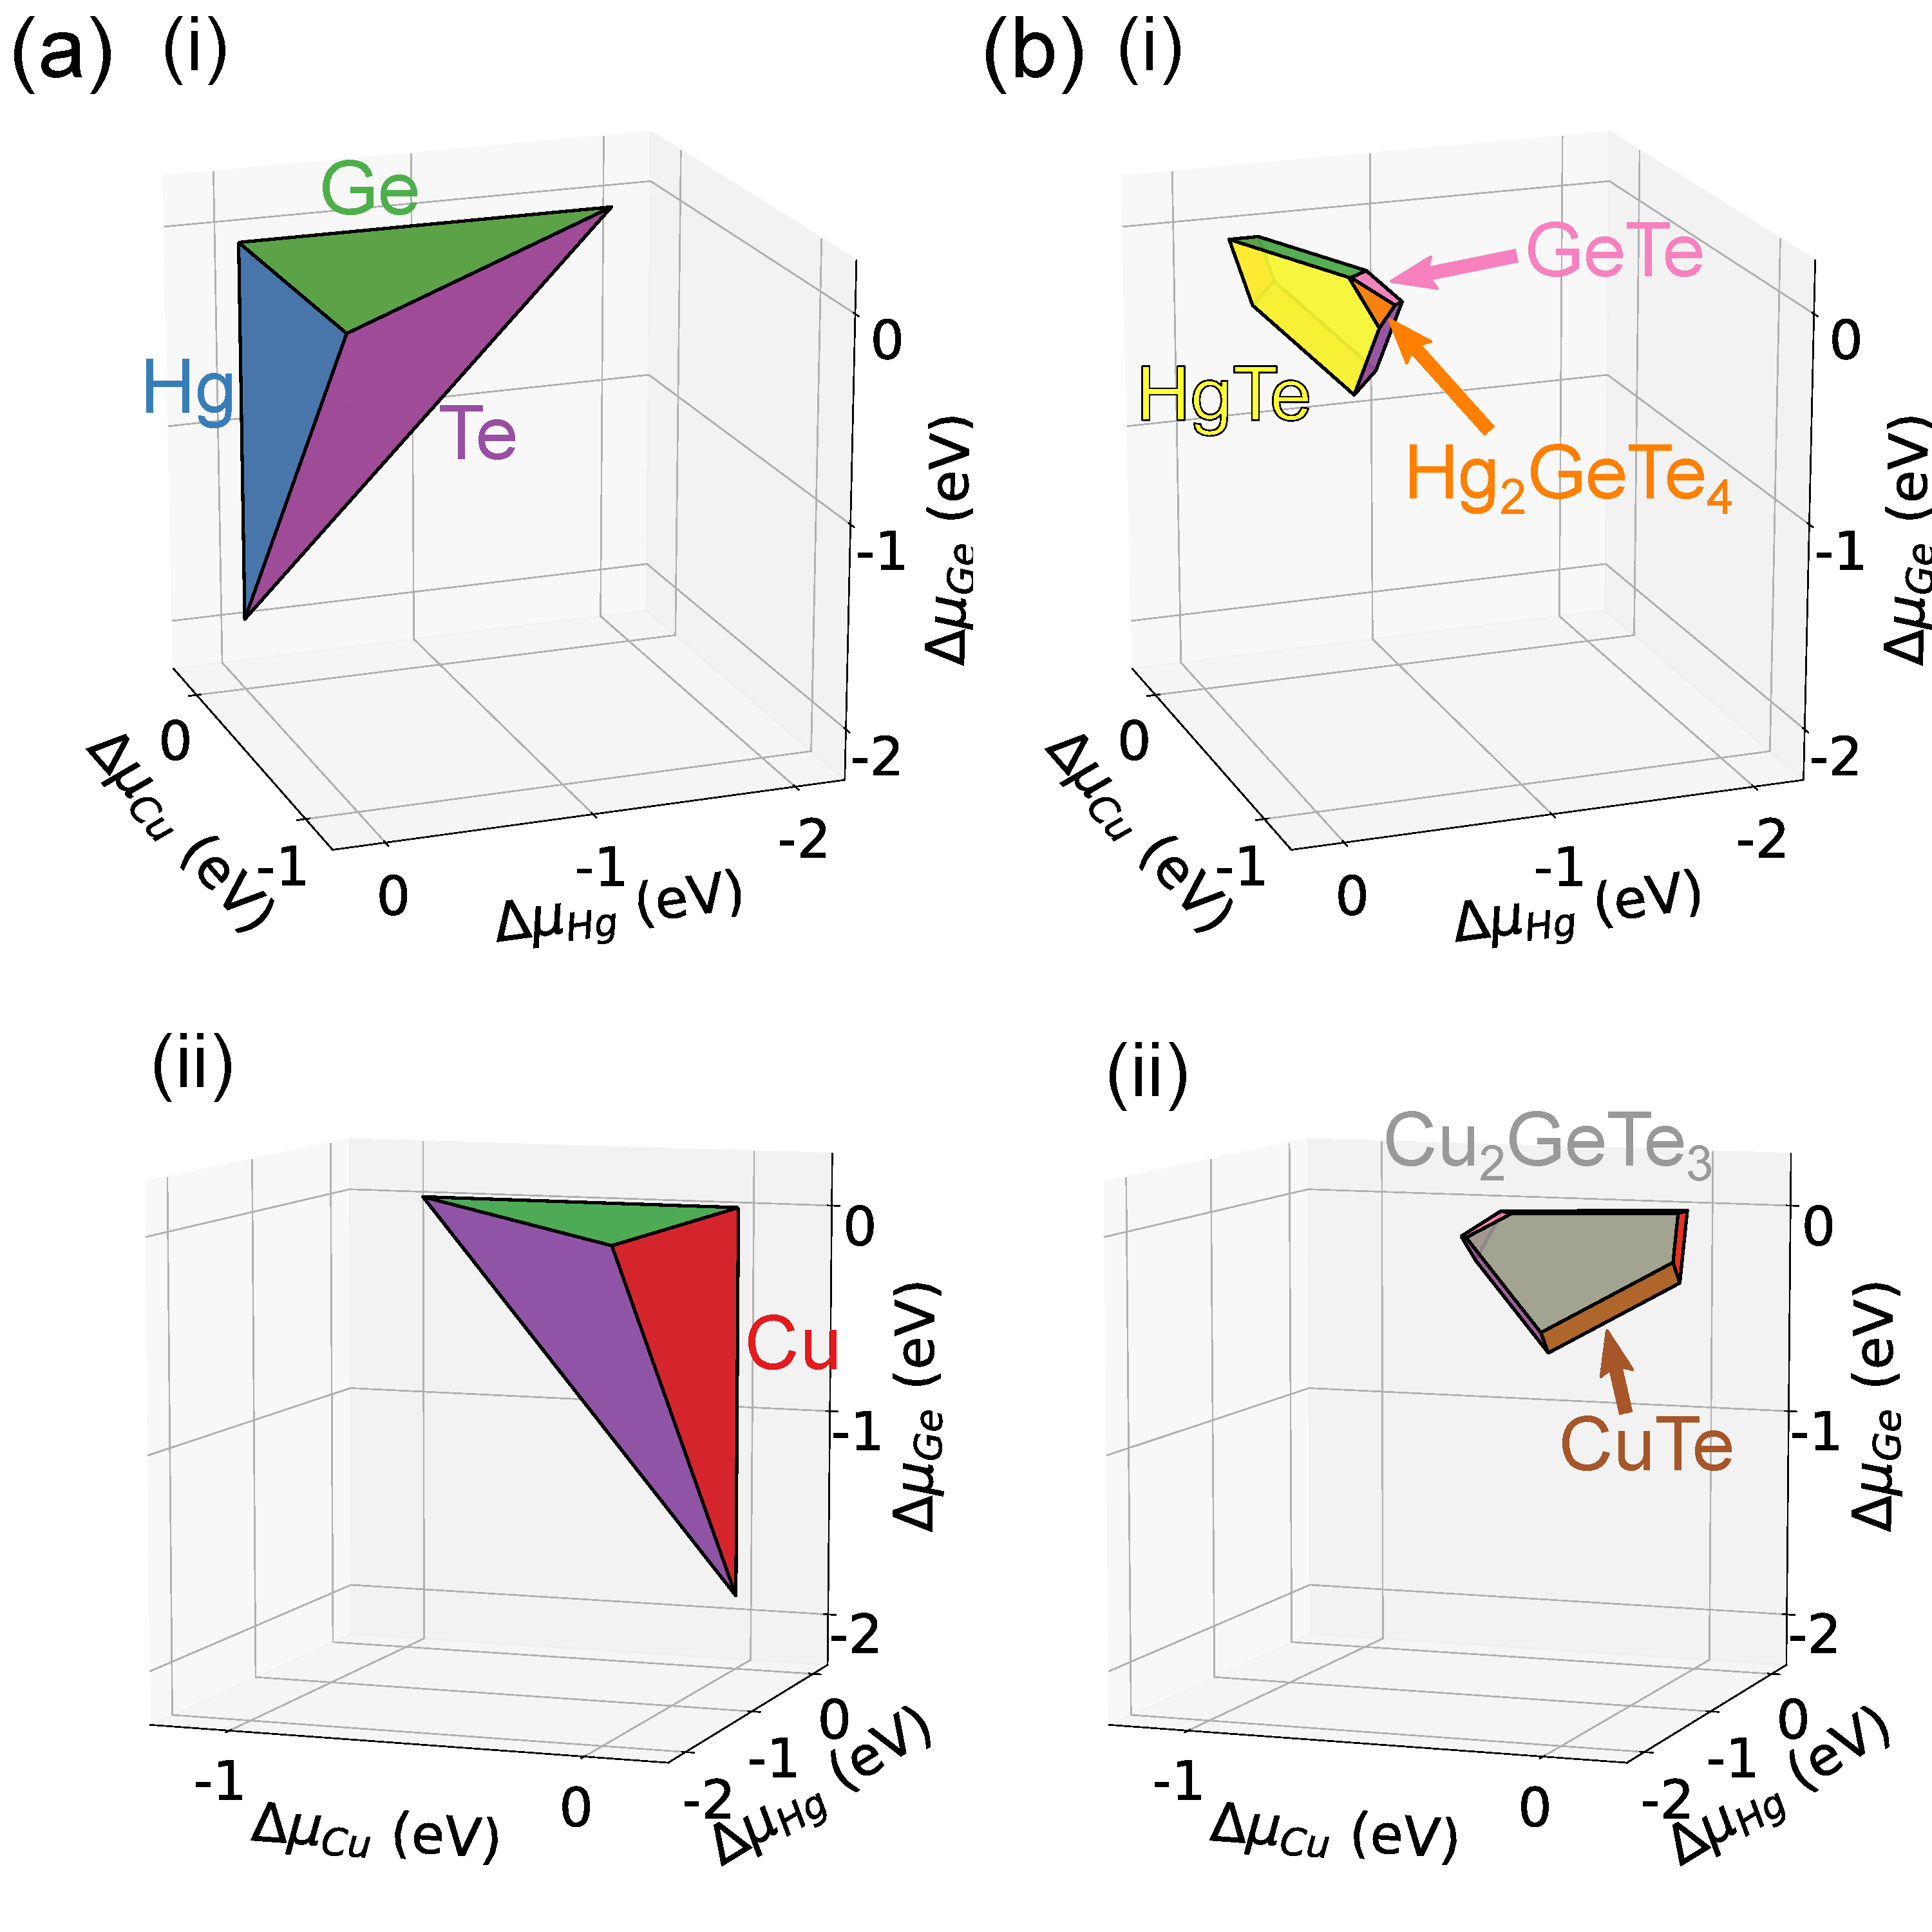
\includegraphics[scale=0.17]{PhaseDiagram_Cu2HgGeTe4_Facets_Labeled.pdf}
    \caption{The phase stability diagram for the  four-component quaternary material Cu$_2$HgGeTe$_4$ contains three degrees of freedom. Here the phase stability diagram is plotted as a function of chemical potentials $\Delta \mu_{Cu}$, $\Delta \mu_{Hg}$, and $\Delta \mu_{Ge}$. Once values for these three parameters are selected, $\mu_{Te}$ becomes fixed. Here, (a,b) show the same plot shown from different viewing orientation. In each case (i) shows the phase stability region bounded only by the constituent elemental phases which takes the form of a pyramid.  Meanwhile, in (ii) each competing compound (binaries and/or ternaries) may remove  some portion of the Cu$_2$HgGeTe$_4$ pyramid and thus introduces a facet according to Equation (\ref{Equation:EnthalpyFormationCompeting}).  Colors correspond to the element/compound that introduces the bound to the phase stability region. \red{For a quaternary material, a four phase equilibrium appears as a point with unique, well-defined chemical potentials, such as ... A line of intersection corresponds to a three phase equilibrium (one degree of freedom), and an area corresponds to a two phase equilibium ...} \blue{[might be nice to indicate some of these on here. also ... do I see a five phase equilibrium for quaternary, Hg2GeTe4, GeTe, and HgTe in (b,i) or is it just the viewing angle?]}}
    \label{Figure:PhaseStability_Schematic}
\end{figure}

Although the formation of ternary and quaternary materials are described by very similar mathematical concepts, the resulting phase stability visualizations are quite different. By Equation (\ref{Equation:EnthalpyFormation}), the stability region of ternary materials is determined by two independent variables, $\Delta \mu_{A^1}$ and $\Delta \mu_{A^2}$, and is therefore described as a plane in three dimensions. Analogously, the stability region of quaternary materials is determined by three independent variables and is therefore described as a solid in three dimensions. VTAnDeM draws the phase stability region of ternary/quaternary materials in three dimensions via a half-space representation of convex polytopes \cite{PyPolyhedron1, PyPolyhedron2}, where the inputs are the inequalities in Equation (\ref{Equation:EnthalpyFormationCompeting}) in the form
\begin{equation}
\begin{aligned}
A x \leq b, \qquad x = (\Delta \mu_{A^1}, ..., \Delta \mu_{A^{n-1}})^{\text{T}}.
\end{aligned}
\label{Equation:HRepresentation}
\end{equation}

Technical difficulties arise however when visualizing and analyzing three-dimensional objects quantitatively, such as determining the range of $\Delta \mu_{A^i}$ values for which $M$ is stable against competing compounds. To mitigate such difficulties, VTAnDeM projects the stability region of a given material $M$ onto two chemical potential axes of the user's choice. We note that while the projection of the stability region of ternary materials is fixed, the shape of the projected stability region for quaternary materials can vary with the chemical potential of the fourth species.

The projection scheme for the quaternary Cu$_2$HgGeTe$_4$ is shown in Figure \ref{Figure:Projection_Schematic}. A slice of the phase stability region corresponds to a value of $\Delta \mu_{\text{Te}}$, and the projection of this slice onto the $\Delta \mu_{\text{Cu}}$-$\Delta \mu_{\text{Hg}}$ is shown as the shaded popup in the left figures. In VTAnDeM, the user can tune the chemical potential of the fourth element using a slider bar, allowing one to probe the entire chemical potential space on a two-dimensional plane.

The phase stability region projected onto two chemical potential axes is calculated internally in VTAnDeM. Once the chemical potential of the fourth species has been fixed ($\Delta \mu_{A^4}'$), a system of inequalities of the form
\begin{equation}
\begin{aligned}
\big( \Delta H^{C_j}_{\text{f}} - b_4 \Delta \mu_{A^4}' \big) - \frac{b_3}{a_3} \big( \Delta H^M_{\text{f}} - a_4 \Delta \mu_{A^4}' \big) \\
\geq \sum_{i=1}^{2} \bigg( b_i - \frac{b_3}{a_3} a_i \bigg) \Delta \mu_{A^i}
\end{aligned}
\label{Equation:EnthalpyFormationProjection}
\end{equation}
is obtained by substituting $\Delta \mu_{A^3}$ of Equation (\ref{Equation:EnthalpyFormation}) into Equation (\ref{Equation:EnthalpyFormationCompeting}). Note that this system of linear inequalities is composed of two variables, $\Delta \mu_{A^1}$ and $\Delta \mu_{A^2}$, so that it bounds a region in two dimensions.

\begin{figure}
    \centering
    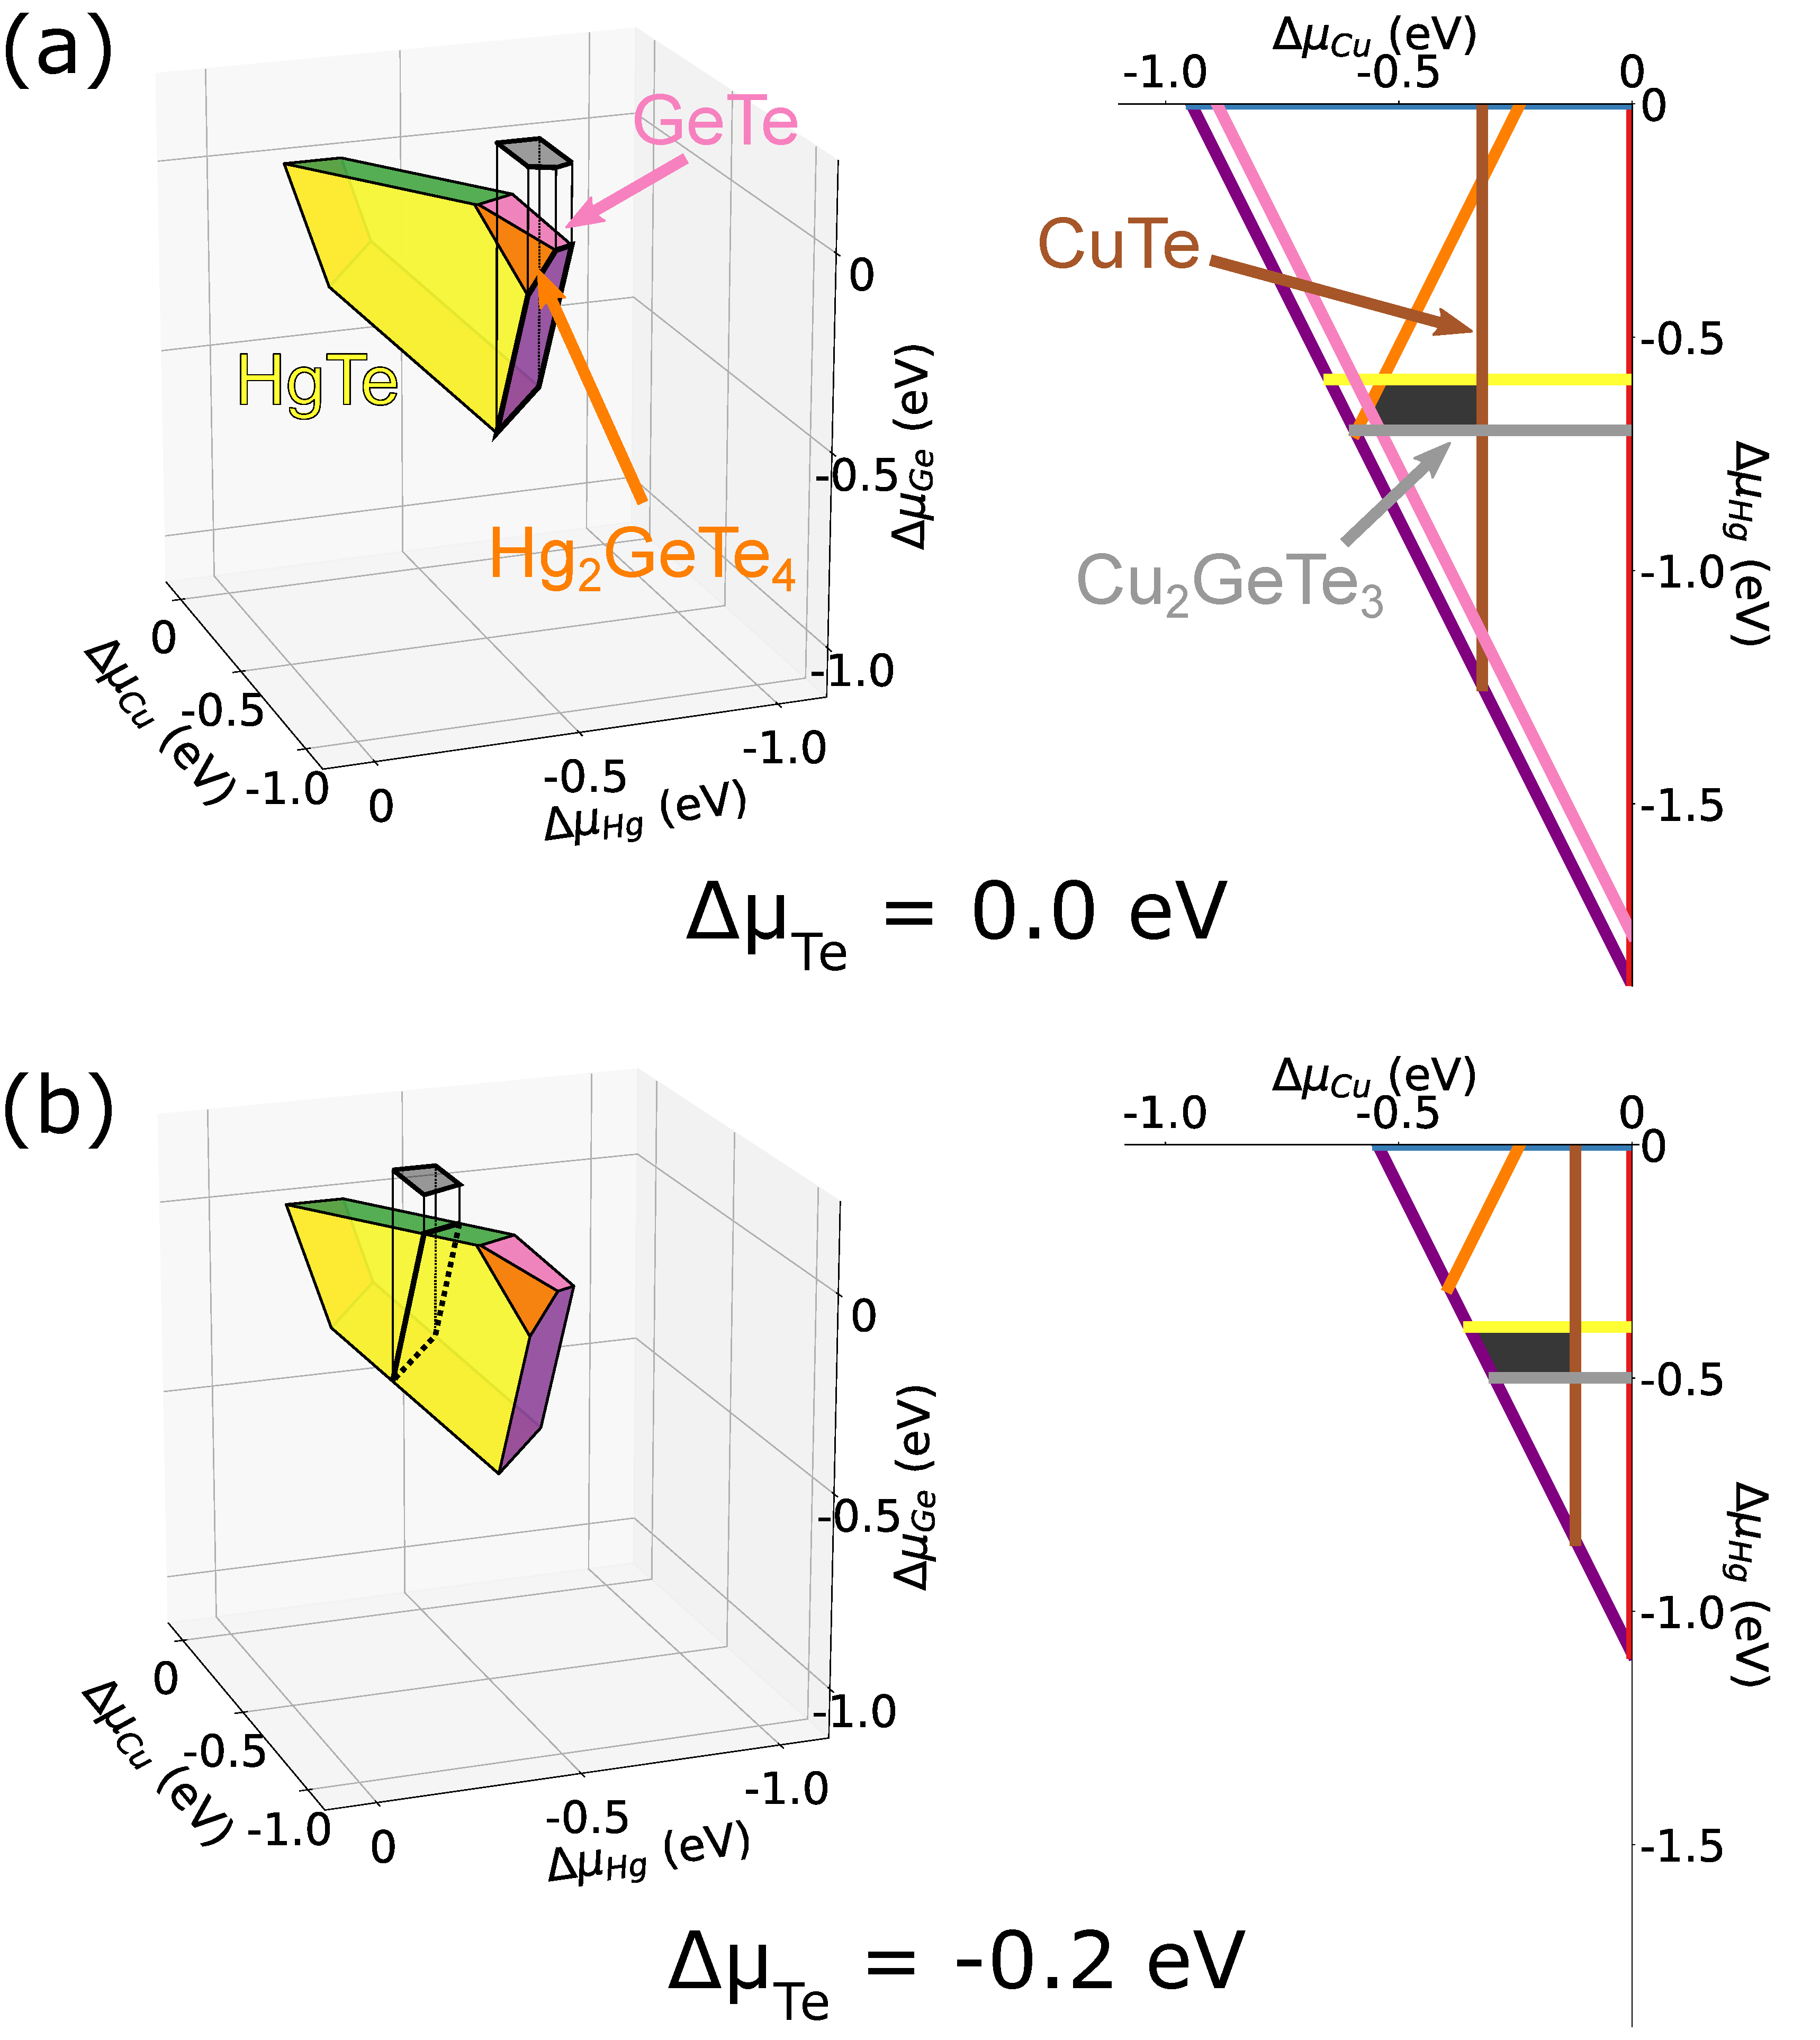
\includegraphics[scale=0.15]{ProjectionSchematic_Cu2HgGeTe4_Project_v3.pdf}
    \caption{Projections of two slices of the three-dimensional volume showing the stability region for Cu$_2$HgGeTe$_4$ onto two dimensions $\Delta \mu_{Cu}$ and $\Delta \mu_{Hg}$. (a)  Projection corresponding to (a) $\Delta \mu_{\text{Te}} = 0.0$ eV, (b) $\Delta \mu_{\text{Te}} = -0.2$ eV, now leaving $\Delta \mu_{Ge}$ as the implied index. Colors represent the competing compounds that bound the stability region. The grey shaded popup on the left  correspond to the grey shaded stability region shown on the right.}
    \label{Figure:Projection_Schematic}
\end{figure}




\subsection{Defect Diagrams}
Defect diagrams convey how the formation energy $\Delta H_{D,q}$ of an isolated point defect $D$ with charge state $q$ varies with the Fermi energy. Within the supercell approach [REF], the defect formation energy is calculated as
\begin{align} \label{Equation:DefectFormationEnthalpy}
\Delta H_{D,q} = E_{D,q} - E_{\text{host}} - \sum_{i} n_i \mu_{A^i} + q E_{\text{F}} + E_{\text{corr}},
\end{align}
where $E_{D,q}$ and $E_{\text{host}}$ are the total energies of the supercell with and without the defect, respectively, $\mu_{A^i}$ is the chemical potential of elemental species $A^i$ as defined in Equation (\ref{Equation:ChemPotDef}), $n_i$ is the number of $A^i$ atoms added ($n_i > 0$) or removed ($n_i < 0$) from the host supercell, $E_{\text{F}}$ is the Fermi energy which ranges between the valence band maximum (VBM) and conduction band minimum (CBM), and $E_{\text{corr}}$ is the correction term that accounts for finite-size corrections within the supercell approach. A schematic for each term contributing to Equation (\ref{Equation:DefectFormationEnthalpy}) is shown in Figure \ref{Figure:DefectFormation}.

\begin{figure*}[ht]
\centering

\includegraphics[width=\textwidth]{DefectFormation.pdf}
\caption{Schematic illustrating the contributions to defect formation energies $\Delta H_{D,q}$. These are (a) the total energy of a system containing the desired defect, (b) the total energy of same system, now without the defect, (c) the number of elements $n_i$ of each species $i$ that must be added to or removed from the pristine supercell to create the defect, and the corresponding chemical potential $\mu_i$, (d) the Fermi energy (electron chemical potential) $E_F$ relevant for defects with charge $q$ arising from exchange of electrons between the defect and the semiconductor, and (e) the finite-size corrections arising from, for example, potential alignment issues and image-charge interactions for charged defects.}
\label{Figure:DefectFormation}
\end{figure*}

Finite-size corrections leading to the $E_{\text{corr}}$ term manifest from several factors \cite{2018_Durrant}. First, a fictitious neutralizing jellium background that compensates for charged defects creates a misalignment in the reference potential. Second, the periodic nature of DFT calculations yield interactions between a defect and its images, which are not present in the dilute limit. Band filling effects of the Moss-Burnstein-type may occur as well in cases where the defect induces a shallow energy state \cite{1954_Moss, 1954_Burnstein}. Various finite-size corrections have been proposed to mitigate these subtle inaccuracies \cite{1995_Makov, 2008_Lany, 2009_Lany, 2009_Freysoldt}. It is worth noting that finite size corrections are not calculated internally by VTAnDeM and are initially listed as $E_{\text{corr}} = 0.0$ in the \textit{Defects\_Tracker.json} file, allowing freedom for the user to use a correction scheme of their choice.



\subsection{Carrier Concentration}
The carrier concentration is derived from charge neutrality, which is dependent on the existence of defects and intrinsic charge carriers. The charge neutrality condition is given by
\begin{align} \label{Equation:ChargeNeutrality}
\sum_{D} q C_{D,q} + p - n = 0,
\end{align}
where $C_{D,q}$ is the concentration of defect $D$ with charge state $q$, and $p$ and $n$ are the hole and electron concentrations, respectively. The concentration of each defect depends on its formation energy by
\begin{align} \label{Equation:DefectConcentration}
C_{D,q}=N_D \text{exp} \bigg(\frac{-\Delta H_{D,q}}{k_B T_{syn}} \bigg)
\end{align}
where $N_D$ is the concentration of $D$ in the crystal structure determined by the multiplicity of Wyckoff sites, $k_B$ is the Boltzmann constant, and $T_{syn}$ is the temperature at which the defects are synthesized. The concentrations of free carriers ($p$ and $n$) on the other hand are contingent on the density of states of the material, where
\begin{align} \label{Equation:HoleConcentration}
p(E_{\text{F}}, T) = \int_{-\infty}^{E_{\text{VBM}}} D_{\text{V}}(\epsilon) [1 - f(\epsilon)] d\epsilon,
\end{align}
and
\begin{align} \label{Equation:ElectronConcentration}
n(E_{\text{F}}, T) = \int_{E_{\text{CBM}}}^{\infty} D_{\text{C}}(\epsilon) f(\epsilon) d\epsilon.
\end{align}
$E_{\text{VBM}}$ and $E_{\text{CBM}}$ are respectively the energies of the VBM and CBM of the electronic band structure, and $D_{\text{V}}(E)$ and $D_{\text{C}}(E)$ are respectively the density of states in the valence and conduction bands. The Fermi-Dirac distribution $f(E)$ describes the probability of a fermionic particle occupying energy level $E$ and is given by the analytic form
\begin{align} \label{Equation:FermiDiracDistribution}
f(E) = \frac{1}{1 + exp\big(\frac{E-E_{\text{F}}}{k_B T}\big)}.
\end{align}

At a fixed temperature, the charge neutrality condition is a monotonic function of the Fermi energy $E_{\text{F}}$. Equation (\ref{Equation:ChargeNeutrality}) is therefore satisfied by a unique Fermi energy, labeled the equilibrium Fermi energy $E_{\text{F}}^{\text{eq}}$, which is determined self-consistently from Equations (\ref{Equation:DefectConcentration})-(\ref{Equation:FermiDiracDistribution}). The hole and electron carrier concentrations are then determined as $p(E_{\text{F}}^{\text{eq}}, T)$ and $n(E_{\text{F}}^{\text{eq}}, T)$, respectively.

It is worth noting that the defect concentration described by Equation (\ref{Equation:DefectConcentration}) neglects entropic and volumetric contributions to the formation energy \cite{2007_Janotti}. The formation entropies of point defects are typically small from changes in the vibrational entropy and are therefore more important at very high temperatures. The volumetric contributions are negligible in the dilute limit.




%\section{Application to Diamond-Like Thermoelectrics} \label{Section_Application_Thermoelectrics}
%Recent work on diamond-like thermoelectric materials, such as chalcopyrite CuInTe$_2$ and stannite Cu$_2$HgGeTe$_4$, have gained increasing interest in not only reducing the lattice thermal conductivity to improve the figure of merit, but also in improving the electrical conductivity through defect engineering \cite{2018_Ortiz, 2019_Ortiz}. As a result, strides towards understanding the effects of common intrinsic defects on the electronic structure of such thermoelectric materials have gained momentum both from experimental and computational perspectives.  In this instance, VTAnDeM serves as a link between DFT-generated thermodynamic/electronic insights of a material and experimental synthesis/characterization inquiries.




\section{Conclusion and Future Outlooks} \label{Section_Conclusion}
We present a post-processing toolkit for simultaneously visualizing phase stability and electronic properties of ternary and quaternary materials. VTAnDeM's visualization capabilities are suitable for numerous materials research areas where phase stability and defect properties crucially underlie material behavior, such as photovoltaics and thermoelectrics. We outline the computational workflow for understanding phase stability and defect properties of materials, and we illustrate the VTAnDeM GUI and database architecture. We also present the mathematical framework of each visualization. The software is currently available on Github under the \textcolor{red}{something} License.

There are several possible future directions regarding VTAnDeM development. For example, VTAnDeM's import functions currently only support VASP calculations, so one possible future work is to include support for other common DFT simulation tools, such as Quantum Espresso and ABINIT. Another feature that VTAnDeM currently lacks is calculating correction energies of defect calculations. Softwares that pre- and post-process DFT defect calculations exist \cite{2017_Goyal, 2018_Broberg, 2018_Naik}, complete with features that calculate the energy corrections. Accordingly, another possible direction is interfacing the VTAnDeM database to read from post-processed outputs by some of these softwares. As VTAnDeM maintains a database of DFT calculations, it may also be helpful for the community to access a global database through a web interface, as done by the TE Design Lab \cite{2016_Gorai}.

\red{To Do: (i) fix carrier concentration issue; (ii) incorporate the synthesis temperature vs. equilibrium analysis; (iii) make web page?; (iv) does this handle binaries?  do we need it to?  maybe not. [others please add to this list]} \blue{[Other points to make somewhere in the text: (i) Defect properties are rarely computed for quaternary systems due to their complexity, but hopefully the automated defect frameworks combined with VTAnDeM visualization will make this more accessible to others now. (ii) need to specify upfront the needed modules/add-ons: polyhedron and pymatgen. anything else? pyQT (iii) state early on that it is currently able to extract needed quantities from VASP output]}


\section*{Acknowledgements} 
This work was supported by the National Science Foundation, Grant No. 1729149. 
M.Y.T. acknowledges the support of the NCSA' Students Pushing INnovation (SPIN) internship program.


\bibliographystyle{unsrt}
\bibliography{bib.bib}

\end{document}
